%% Undergraduate thesis paper
%%
%% M E M E R A T O R
%%
%% Author: AlOrozco53
%% Advisor: ivanvladimir
%% Version: 0.0
\documentclass[letter]{book}
\usepackage[utf8]{inputenc}
\usepackage[T1]{fontenc}
\usepackage{graphicx}
\usepackage[spanish]{babel}

\graphicspath{{img/}} %% image directory

\begin{document}

\thispagestyle{empty}

\frontmatter

\begin{titlepage}
  \begin{minipage}{.3\textwidth}
    \flushleft
    \center{
\includegraphics[scale=.09]{unam.pdf}}
    \vspace{20pt}
    \center{
      \rule{.5pt}{.6\textheight}
      \hspace{7pt}
      \rule{2pt}{.6\textheight}
      \hspace{7pt}
      \rule{.5pt}{.6\textheight}
    }\\
    \center{
\includegraphics[scale=.22]{ciencias.pdf}}
  \end{minipage}
  \begin{minipage}{.7\textwidth}
    \flushright
    \center{
      \center{
        \LARGE{U}\large{NIVERSIDAD} \LARGE{N}\large{ACIONAL}
        \LARGE{A}\large{UTÓNOMA} \\[10pt]
        \large{DE}
        \LARGE{M}\large{ÉXICO}
      }\\
      \rule{\textwidth}{2pt}
      \\
      \hrulefill\\[1cm]
      \LARGE{F}\large{ACULTAD DE } \LARGE{C}\large{IENCIAS}\\[2cm]
      \large{
        Generación automática de memes de Internet a través de una red neuronal profunda  }\\[2cm]
      \huge{
        T \hspace{1cm} E \hspace{1cm} S \hspace{1cm} I \hspace{1cm} S  }\\[1cm]
      \large{QUE PARA OBTENER EL TÍTULO DE:}\\[1cm]
      \large{
        Licenciado en Ciencias de la Computación  }\\[1cm]
      \large{PRESENTA:}\\[1cm]
      \large{
        Albert Manuel Orozco Camacho  }\\[1cm]
      \large{
        TUTOR  }\\[1cm]
      \large{
        Dr. Ivan Vladimir Meza Ruiz  }
    }
  \end{minipage}
\end{titlepage}

\tableofcontents

\mainmatter

\begin{savequote}[45mm]
  When you plant a fertile meme in my mind you literally parasitize my brain,\
  turning it into a vehicle for the meme's propagation in just the way that a\
  virus may parasitize the genetic mechanism of a host cell.
  \qauthor{Richard Dawkins \cite{dawkins2006}}
\end{savequote}

\chapter{Introducción}

\noindent
El siglo XXI ha traido consigo una transformación radical en las formas de comunicación\
entre personas. Hoy en día, el uso de redes sociales \emph{democratiza} el acceso\
a la información más relevante ocurriendo en tiempo real, sin tener que esperar a que un medio\
masivo publique una noticia sobre ello. Cualquier persona con una cuenta de \textit{Twitter} puede\
tomar una fotografía, subirla a la \textit{web} y etiquetarla de la manera en que más le convenga (mediante\
\textit{hashtags}, por ejemplo). Dependiendo de muchos factores, incluyendo el alcance del\
\textit{tuit} y el número de seguidores de la cuenta de Twitter, es posible que la imagen se vuelva\
más popular de lo que una nota publicada por algún periodista serio pueda alcanzar.\par
Este fenómeno también se explica por las intenciones que llevan a la gente a interactuar dentro de\
las redes sociales. Al usuario se le da la libertad de hacer que el contenido de su \textit{timeline (TL)}\
sea tan ocioso, o tan serio, como éste quiera, siguiendo en el caso de Twitter. Cuando un tuit acompañado\
de una imagen se vuelve \emph{viral}, surge un fenómeno de propagación en el cual el poder del\
\textit{tuitero} permite re-etiquetar la imagen sin perder la esencia de la idea original transimitida\
por la misma.\par
En general, este fenómeno no es exclusivo de Twitter y ha ocurrido en Internet desde que la comunicación\
entre personas se efectuaba exclusivamente por medio de correos electrónicos. Para englobar a las diversas\
maneras en las que se viraliza cierta infomación en la web en un solo concepto, se ha popularizado el\
término \emph{\textbf{meme (de Internet)}}, el cual pretende \emph{discretizar} la información cultural\
en unidades capaces de pasar de persona a persona, gradualmente escalar en un fenómeno social compartido\
e incluso \emph{evolucionar} \cite{shifman2014}.\par
Paralelamente, el constante incremento en el uso de redes sociales genera un cúmulo de datos esparcidos\
por el Internet. De acuerdo al un estudio descrito en \cite{website:smartinsights} y publicado en 2016,\
el $46\%$ de la población mundial son usuarios de Internet y el $31\%$ son usuarios activos de alguna red social.\
Además, durante 2015 se produjo un aumento de usuarios equivalente a $10\%$ en los dos rubros descritos anteriormente.\
Consecuencia de esto es que a diario, el intercambio de información favorece en la riqueza y complejidad\
de nuevas ideas que se acumulan en grandes servidores pero cuya relevancia está empezando a ser explorada.\par
Dentro de la rama de las ciencias de la computación, conocida como \textbf{inteligencia artificial}, el\
\textbf{aprendizaje automático} (\emph{machine learning} en inglés) propone técnicas capaces de lograr que, a partir\
de grandes cantidades de datos, un sistema de cómputo revele información oculta para muchos seres humanos.\
El auge del subconjunto de \emph{algoritmos de aprendizaje} automático conocido como\
\textbf{aprendizaje profundo} (\emph{deep learning} en inglés), trae consigo un importante adelanto\
en el desempeño de computadoras al realizar habilidades humanas. Dos ejemplos significativos incluye el reconocimiento\
de imágenes y rostros mediante visión computacional y la generación automática de texto coherente en algún idioma.\par
Motivado por lo establecido en los párrafos anteriores, en el presente trabajo se explorarán dos modelos de\
aprendizaje profundo para entrenar, identificar y, finalmente, etiquetar memes de Internet. Se considerará únicamente\
el caso de una imagen (la cual, en el la mayoría de los casos, incluye a un solo personaje) y una \emph{leyenda} asociada.\
Por lo tanto, se presentará un método para hacer que la computadora aprenda al personaje dentro del meme y la información\
textual que transmite; posteriormente se experimentará etiquetando memes no antes vistos por dicha computadora.

\section{Memes de Internet y \emph{memética}}

\noindent
El término \emph{meme} fue acuñado por el biólogo Richard Dawkins en su libro \emph{``The Selfish Gene''}\
de 1976. Mediante una analogía con el papel del \emph{gen} en la evolución darwiniana, Dawkins\
propuso una teoría cultural en la cual el meme es visto como la unidad que se propaga por generaciones\
y sobrevive mediante un proceso semejante a la selección natural. Dawkins conjeturó que la teoría de la evolución\
de Darwin es una instancia particular de un proceso que se puede encontrar en otras áreas; en particular,\
es suficiente que cualquier concepto que incorpore las propiedades de \emph{longevidad}, \emph{fecundidad} y\
\emph{fidelidad de copias} para que éste tenga un comportamiento evolutivo a través del tiempo \cite{distin2005}.\par
Hoy en día, se le conoce como \emph{meme} principalmente al objeto proveniente de Internet y que incorpora,\
en el mayor de los casos, una imagen y una leyenda que cuenta algo sobre la imagen. Es importante recalcar\
el aspecto humorístico, muchas veces incluso irónico, que caracteriza al meme de la actualidad ya que ello\
contribuye a la difusión de los mismos por la web. Sin embargo, es el diseño \emph{centrado al usuario} característico\
de la llamada \emph{Web 2.0} lo que mayormente facilita la propagación de memes.\par
Dentro de esta estructura tecnológica, las tres propiedades adscritas por Dawkins a cualquier objeto evolutivo se\
satisfacen para los memes: la digitalización permite una transmisión casi sin interferencias (fidelidad de copias),\
el número de copias compartidas en una unidad de tiempo es incremental -- dada la facilidad de compartir información\
``de nodo a nodo'' -- (fecundidad) y el aumento en la longevidad de la información es respaldado por la capacidad de\
almacenamiento indefinido en los servidores de la web. \href{http://www.reddit.com}{\texttt{Reddit.com}} es uno\
de los sitios web con mayor flujo y contenido de memes; su eslogan \emph{``the front page of the Internet''}\
resume la importancia cultural que el alcance de su contenido modifica las formas de obtener y discutir información\
de cualquier índole. Lo que Dawkins no se imaginó en los años 70's es que el meme se convertiría en la mejor\
manera de encapsular los aspectos más fundamentales de Internet \cite{shifman2014}.

\begin{figure}
  \centering
  
\includegraphics[width=0.5\textwidth]{success_kid}
  \caption{Clásico ejemplo de un personaje \emph{memificado} junto con una de sus
    leyendas (descripciones). Tomado de \href{http://www.memegenerator.net}{MemeGenerator.net}
    \cite{website:memegenerator:kid}.
  }
\end{figure}

La trascendencia del concepto de Dawkins provocó el surgimiento de la \emph{memética}, la disciplina\
sociobiológica que extrapola el concepto de evolución de la teoría de Darwin para colocar al\
meme como instrumento de supervivencia, un \emph{replicador}. Originalmente, Dawkins sugirió como\
ejemplos de memes a frases pegadizas, tonos de audio, modas, habilidades o simplemente ideas.\
Más aún, según Dawkins el meme es una ``unidad de información que reside en un cerebro'' \cite{dawkins2006},\
una afirmación que sugiere la relevancia que el alcance de las redes sociales tiene en la población\
actual, incluso mayor a la que otros medios de comunicación -- como la televisión o la radio -- alcanzaron\
desde su concepción.

\section{Un esbozo sobre las redes neuronales profundas}

\section{Objetivos de la tesis}

\chapter{Trabajo Relacionado}

TODO

\chapter{Aprendizaje Profundo}

TODO

\chapter{Red neuronal para descripciones de memes}

\noindent
\lettrine[lines=2, lhang=0.33, loversize=0.25]{\textbf{D}}{ejando}\
de lado la teoría memética introducida por Dawkins \cite{dawkins2006}, consideraremos a\
un \emph{meme} de forma abstracta, separando su representación visual de su leyenda.\
Por consecuencia, la arquitectura neuronal que se presentará en este capítulo,\
tratará de procesar los siguientes tipos de datos:
\begin{itemize}
\item Un \emph{tensor} con dimensiones \verb+[w, h, 3]+
  \footnote{
    Aquí, usamos la notación del paquete \href{http://www.numpy.org}{NumPy}\
    del lenguaje de programación \emph{Python} para referirnos a las dimensiones\
    de un tensor.
  }, donde \verb+w+ y \verb+h+ son el ancho y el largo de una imagen, mientras que\
  el 3 simboliza los canales de la misma (RGB).
\item Un vector que contiene los índices correspondientes a las palabras de una leyenda;\
  éstos se obtienen \textit{mapeando} números naturales con un diccionario que reúne todas
  las palabras del conjunto de datos de entrenamiento.
\end{itemize}

\section{Formalización del problema de aprendizaje}

\noindent
Los recientes avances en generación de descripciones de imágenes destacan el éxito\
de una CNN que obtiene una representación vectorial de las características más\
importantes de las imágenes de entrenamiento\cite{DBLP:journals/corr/VinyalsTBE14}.\
Vinyals, \emph{et al}, además proponen canalizar estos vectores hacia una arquitectura recurrente\
que, junto con las descripciones de las mismas creen un modelo de lenguaje\
\footnote{
  Llamamos \textbf{modelo de lenguaje \textit{probabilístico}} a una distribución de\
  probabilidad sobre todos los enunciados formados por las palabras de un diccionario.\
  Un buen modelo de lenguaje debe de maximizar la \emph{probabilidad conjunta} enunciados\
  que sean coherentes sintáctica y semánticamente.
}.\par
La comunidad de procesamiento de lenguaje natural se ha \emph{inspirado} en el modelo de\
\emph{traducción automática neuronal} que incorpora una LSTM, cuya memoria inicial está dada por\
los vectores salientes de la CNN, que codifica un enunciado de entrada de longitud indefinida\
en una representación de longitud fija para, posteriormente, ``decodificar'' ésta última en\
un enunciado objetivo. Intuitivamente, se puede pensar en una máquina abstracta que, dadas las\
características de una imagen intenta ``traducir'' las palabras $S_1,\ldots,S_t$ (un prefijo\
de la imagen) para obtener el sufijo $S_{t+1},\ldots,S_{N}$.\par
Formalmente, estamos construyendo dos distribuciones de probabilidad dadas por la CNN y la LSTM,\
respectivamente. El problema, en cuestión, de aprendizaje automático consiste en maximizar\
la \emph{verosimilitud} de la descripción correcta de una imagen $I$ por un enunciado $S$:
\begin{equation}
  \theta^* = \argmax_\theta \sum_{I, S} \log p(S|I;\theta)
\end{equation}
donde $\theta$ son los parámetros del modelo. En este caso, $S$ representa a cualquier enunciado\
sin restricción de longitud; para fijar su longitud, hacemos uso de la regla de la cadena\
probabilística para calcular la $\log$-probabilidad de $S = S_0,\ldots,S_N$:
\begin{equation}
  \log p(S|I) = \sum_{t=0}^N \log p(S_{t+1}|I,S_0,\ldots,S_t).
\end{equation}
Obsérvese que la dependencia de los parámetros $\theta$ continúa aunque no se haga explícito.\par
En otras palabras, proponemos usar una LSTM para estimar $p(S_{t+1}|I,S_0,\ldots,S_t)$, de acuerdo\
al \emph{estado del arte} actual de tareas de predicción de secuencias de símbolos. La tupla\
$(I,S)$, será uno de los tantos ejemplares de entrenamiento, donde la imagen $I$ son las características\
encontradas por una CNN ajustadas a un espacio vectorial. Este esquema neuronal garantiza\
un aprendizaje \emph{de punto a punto}, es decir, la red tendrá la capacidad de considerar cada pixel\
de una imagen para determinar qué tanto contribuye en la generación de enunciados.

\section{Inception \emph{v.3}}

\begin{center}
  \emph{¿Cuántas capas son necesarias y suficientes?}
\end{center}\par
\noindent
Nos referimos a una CNN como \textbf{incrustadora} o \textbf{encajadora} (\emph{embedder} en inglés)\
pues su trabajo consiste en extraer las características de una imagen y comprimirlas en un espacio\
vectorial fijo. Sabemos, a partir del capítulo anterior, de la capacidad de filtrar detalles de una\
capa convolucional; sin embargo no existe pista alguna que nos muestre con exactitud qué hay que\
tomar en cuenta de un conjunto de imágnes de entrenamiento (¡y sobre todo de memes!).\par
Este problema se reduce al de la construcción de una arquitectura suficientemente \emph{general} que\
sea capaz de filtrar hasta el más mínimo detalle de una imagen. Con el fin de atacarlo,\
surgió la competencia anual \emph{``Large Scale Visual Recognition Challenge''} (ILSVRC), cuyo\
objetivo ha sido el de mejorar en la tarea general de etiquetamiento de imágenes. Aunado a ello, el laboratorio\
de visión computacional de Stanford University comparte el conjunto de datos \emph{ImageNet} que reúne\
14,197,122 imágenes etiquetadas para el entrenamiento y la evaluación de los algoritmos participantes.\par
En 2014, los modelos neuronales de gran profundidad comenzaron a ganar popularidad en esta tarea, sobre\
todo por el desempeño de la arquitectura \textbf{Inception} \cite{DBLP:journals/corr/SzegedyVISW15}.\
A diferencia de algunas de sus predecesoras (GoogLeNet, AlexNet, VGGNet), Inception reduce hasta 12 veces\
el número de parámetros (pesos) requeridos, garantizando un desempeño computacional más óptimo. Es decir,\
su escalabilidad le permite incorporarse a la industria de grandes bases de datos. Por ello, se ha decidido\
usar a Inception como ``incrustadora'' de imágenes.\par
Aquí, vale la pena destacar que la profundidad que posee Inception es del orden de 256 capas y que\
algunas de sus predecesoras se caracterizaban por una profundidad de al menos un orden de magnitud\
(exponencial) a ella. Sin embargo, la reducción en la amplitud promedio (número de dimensiones por capa)\
le permite remover algunos cuellos de botella de desempeño. A continuación, se presentan algunos\
de los principios de diseño de Inception.
\begin{enumerate}[label=\textbf{S.\arabic*}]
\item Dos capas contiguas, con un número de neuronas conectadas menor al promedio entre cualesquiera\
  otras, implican que la información está siendo comprimida mientras fluye hacia la capa de salida.\
  En general, se busca capturar la mayor cantidad de detalles, a través de un número considerable de\
  dimensiones en las primeras capas; por lo que, más o menos, el número de dimensiones debe reducirse\
  de a poco desde el inicio hasta el final.
\item Se prefiere incrementar el número de ``capas de activación'' por cada grupo de convoluciones-pooling,\
  pues esto revela una cantidad mayor de características y facilita el entrenamiento.
\item \label{sp-agg} Es posible realizar una operación de \emph{adición espacial}, en la cual se combinen incrustaciones\
  con dimensiones bajas. Más aún, se pueden realizar reducciones dimensionales tras alguna adición espacial\
  y previamente a una convolución, sin pérdida de información.
\item El balance entre la amplitud y la profundidad de la red neuronal contribuye directamente a la calidad\
  del desempeño de la misma. Sin embargo, ambas medidas deben de ser incrementadas en paralelo, para\
  garantizar un aumento \emph{constante} en el costo computacional de la red.
\end{enumerate}

\subsection{Factorización de convoluciones}

Reducción de dimensiones, en una red convolucional, implica reducción \emph{significativa} de parámetros (de pesos)\
por capa convolucional. Una de las técnicas usadas, primero por GoogLeNet
\footnote{
  Para más información sobre la arquitectura de \emph{GoogLeNet}, revisar \url{https://arxiv.org/abs/1409.4842}.
},
y luego adoptada por Inception consiste en \textbf{factorizar} (\emph{descomponer}) una capa CONV con un filtro\
``grande'' en varias capas CONV adyacentes que cuya suma de las dimensiones de sus respectivos filtros sea\
equivalente a la capa factorizada.\par

\begin{figure}[H]
  \centering
  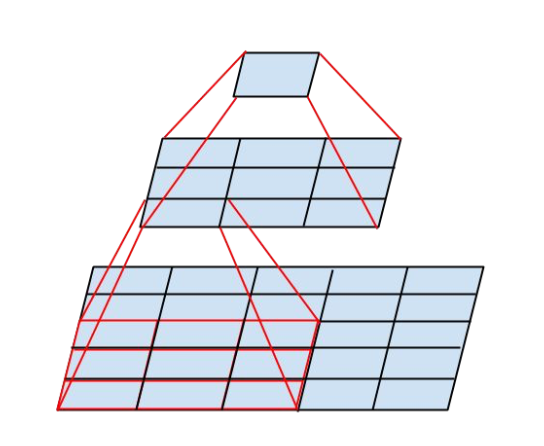
\includegraphics[width=0.6\textwidth]{conv-to-mlp}
  \caption{Una convolución de $5 \times 5$ es un perceptrón multicapa, \emph{per se}.
    (Tomado de \url{https://arxiv.org/pdf/1512.00567.pdf}.)}
  \label{conv-to-mlp}
\end{figure}

La reducción de parámetros por capa CONV implica, además, un entrenamiento más rápido. El costo radica en aplicar\
más convoluciones por cada capa CONV cuyo filtro tiene dimensiones \emph{considerablemente} grandes. Para\
profundizar más en esta idea, imaginemos un filtro de $5 \times 5$. Uno de los beneficios que trae consigo\
el tener una filtro de tamaño ``grande'' (por conveniencia, aquí así lo consideramos) es que la cobertura del\
mismo sobre una imagen le permite capturar mayores detalles de la misma. Ahora, recordemos que una capa CONV\
puede ser vista como un MLP, como se vio en el capítulo anterior; en realidad, ¡el filtro en cuestión\
es una capa totalmente conectada que pasa por toda la imagen de entrada! ¿Por qué no descomponer este MLP\
en varios filtros pequeños aplicados de manera \emph{paralela} sobre la imagen? El resultado es la\
factorización en dos filtros de $3 \times 3$ como se muestra en la figura (\ref{conv-to-mlp}).\par

\begin{figure}[H]
  \centering
  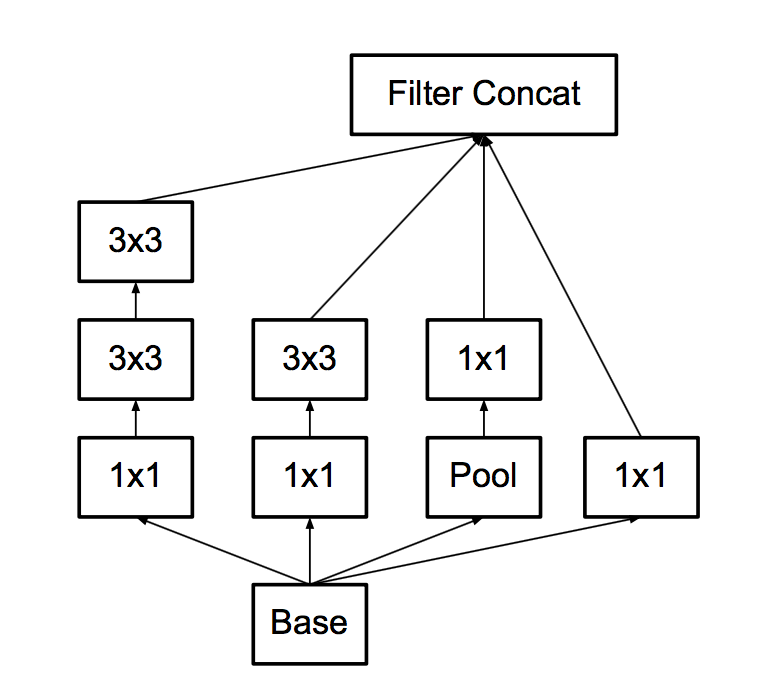
\includegraphics[width=0.6\textwidth]{factorization}
  \caption{Otra manera de factorizar una convolución consiste en paralelizar el cómputo del filtro.
    Cabe destacar que los parámetros de cada nuevo filtro son \emph{compartidos} entre sí,\
    por cada nueva capa. Aquí reemplazamos un filtro de $5 \times 5$ con dos filtros de $3 \times 3$
    y una capa de pooling.
    (Tomado de \url{https://arxiv.org/pdf/1512.00567.pdf}.)}
  \label{factorization}
\end{figure}

En términos propios de la teoría de lenguajes de programación, podemos afirmar que una red neuronal, vista como un\
lenguaje formal, posee una estructura que le permite ser construida de manera \emph{inductiva} a partir\
de pequeñas entidades \emph{bien} definidas. ¿Cómo es que, entonces, se optimiza una red CNN? Minimizando la complejidad\
del cómputo de sus estructuras básicas. En este caso, aprovechamos el cómputo paralelo para factorizar un\
filtro, de donde surgen varios ``hilos de ejecución'' en el grafo de la misma que, deberán ser\
eventualmente \emph{concatenados} en un solo tensor resultante.\par
A la estructura presentada en la figura (\ref{factorization}), se le denomina comúnmente como módulo\
\emph{Inception}. Por otro lado, decimos que una convolución con un filtro de $1 \times 1$ procesa\
\emph{localmente} una imagen de entrada pues realiza una activación (filtrado) exhaustiva a nivel\
de pixeles individuales. En contraste, siguiendo el principio de diseño (\ref{sp-agg}), la reducción\
una adición espacial incorpora dos o más entradas en una. La reducción de dimensiones toma un papel\
clave para garantizar que no haya pérdida de información. No obstante, un incremento en tasa de procesamientos\
locales contra adiciones espaciales favorece la existencia de representaciones dispersas de dimensiones\
altas.

\begin{figure}[H]
  \centering
  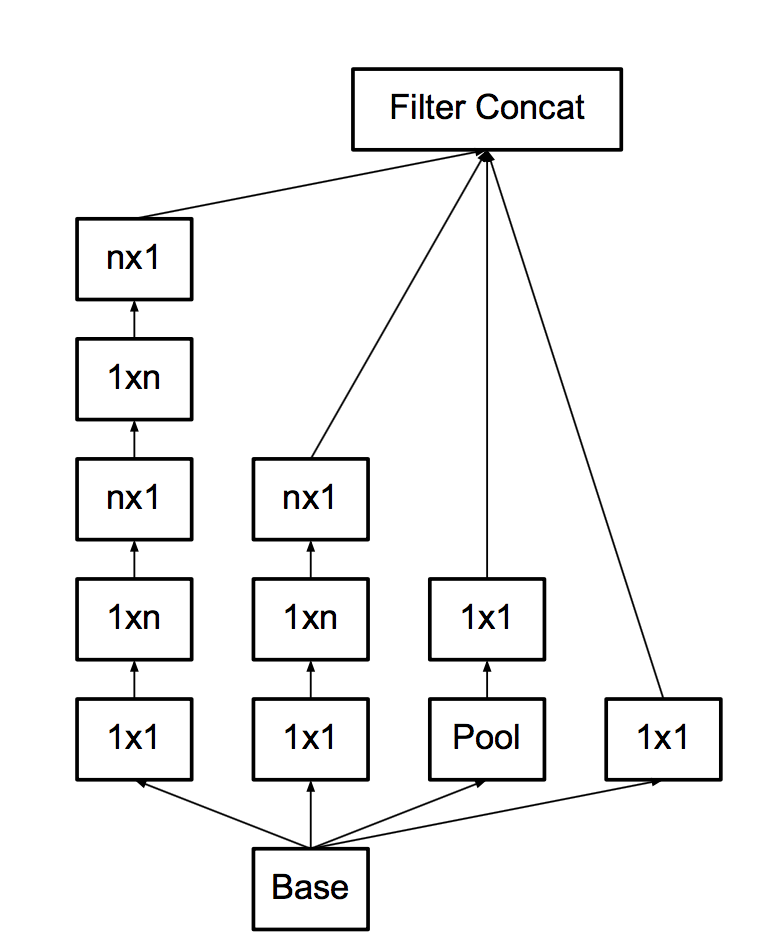
\includegraphics[width=0.6\textwidth]{factorization2}
  \caption{Factorización de una convolución de $n \times n$, donde $n = 7$.
    (Tomado de \url{https://arxiv.org/pdf/1512.00567.pdf}.)}
  \label{factorization2}
\end{figure}

\begin{figure}[H]
  \centering
  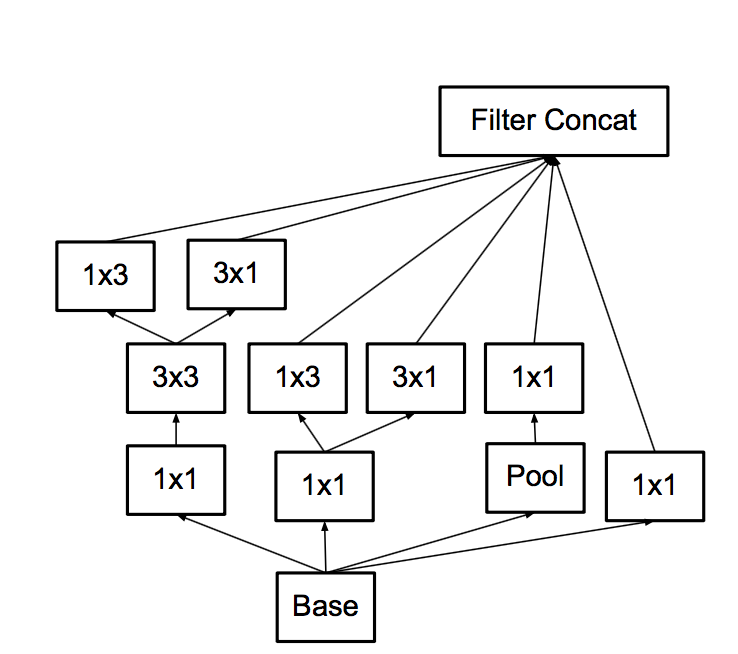
\includegraphics[width=0.6\textwidth]{factorization3}
  \caption{Factorización de una convolución de $8 \times 8$.
    (Tomado de \url{https://arxiv.org/pdf/1512.00567.pdf}.)}
  \label{factorization3}
\end{figure}

Para concluir con esta sección, presentamos las capas que constituyen a la arquitectura Inception\
en la siguiente tabla.

\noindent
\resizebox{\textwidth}{!}{
  \begin{tabular}{|l|c|c|}
    \hline
    \textbf{tipo} & \textbf{tamaño de filtro / zancada} & \textbf{tamaño de la entrada}\\
    \hline \hline
    CONV & $3 \times 3 / 2$ & $299 \times 299 \times 3$ \\
    \hline
    CONV & $3 \times 3 / 1$ & $149 \times 149 \times 32$ \\
    \hline
    CONV con relleno de ceros & $3 \times 3 / 1$ & $147 \times 147 \times 32$ \\
    \hline
    POOL & $3 \times 3 / 2$ & $147 \times 147 \times 64$ \\
    \hline
    CONV & $3 \times 3 / 1$ & $73 \times 73 \times 64$ \\
    \hline
    CONV & $3 \times 3 / 2$ & $71 \times 71 \times 80$ \\
    \hline
    CONV & $3 \times 3 / 1$ & $35 \times 35 \times 192$ \\
    \hline
    $3 \times$ Inception & figura (\ref{factorization}) & $35 \times 35 \times 288$ \\
    \hline
    $5 \times$ Inception & figura (\ref{factorization2}) & $17 \times 17 \times 768$ \\
    \hline
    $2 \times$ Inception & figura (\ref{factorization3}) & $8 \times 8 \times 1280$ \\
    \hline
    POOL & $8 \times 8 / 2$ & $8 \times 8 \times 2048$ \\
    \hline
    LINEAL & logits ($\log$-probabilidades) & $1 \times 1 \times 2048$ \\
    \hline
    MLP-SOFTMAX & clasificador & $1 \times 1 \times 1000$ \\
    \hline
  \end{tabular}
}

\section{Poniendo todo junto}

\noindent
Esencialmente, la estructura de cada unidad LSTM usada en la implementación de la RNN es la misma\
que la que fue presentada en la última sección del capítulo anterior. Lo único que cambia es la\
incorporación del tensor de la penúltima capa de Inception ($CNN(I)$), como memoria inicial ($h^{(0)}$).\par
El entrenamiento de la LSTM se lleva a cabo \emph{desenvolviendo} la recurrencia en un tamaño\
fijo de copias de la LSTM (digamos, $N$). En el tiempo $t+1$, se calcula la probabilidad que tiene\
cada palabra en el diccionario de ser $S_{t+1}$ a partir de $p(S_t|I,S_0,\ldots,S_{t-1})$.\
En resumen,
\begin{align}
  x_{-1} &= CNN(I)\\
  x_t &= W_eS_t,\ \ t \in \{0,\ldots,N-1\}\\
  p_{t+1} &= LSTM(x_t),\ \ t \in \{0,\ldots,N-1\}
\end{align}
donde $x_{-1}$ indica la primera entrada de la LSTM, $x_t$ son las entradas subsecuentes,
$W_e$ es un tensor que incrusta la palabra $S_t$ en el mismo espacio vectorial que $CNN(\cdot)$ y\
$p_{t+1}$ es el tensor de $\log$-probabilidades por cada palabra en el diccionario en el tiempo $t+1$.\
Cabe destacar que $S_t$ se representa matricialmente como un vector codificado \emph{en caliente}
\footnote{
  En una codificación \textbf{en caliente} (\emph{one-hot encoding}, en inglés), se aplica la\
  función indicadora sobre un vector con la dimensión del diccionario de palabras, dejando un 1\
  en el índice que corresponde a la palabra $i$ y 0 en cualquier otro.
}.\par
El error de la arquitectura se calcula mediante la verosimilitud logarítmica negativa,\
sumando cada palabra:
\begin{equation}
  L(I, S) = - \sum_{t=1} ^N \log p_t(S_t). 
\end{equation}
Acto seguido, se minimiza este error con respecto a todos los parámetros de la LSTM, la penúltima\
capa de la CNN y las incrustaciones $W_e$.\par
Finalmente, para la generación de enunciados se utiliza el algoritmo de \textbf{búsqueda por haces}\
(\emph{beam search} en inglés). Iterativamente, se considera el conjunto de las $k$ mejores palabras\
que son candidatas para ser $S_t$ en el tiempo $t$. Esto es una aproximación de
\begin{equation}
  S = \argmax_{S'} p(S'|I)
\end{equation}

\begin{figure}[H]
  \centering
  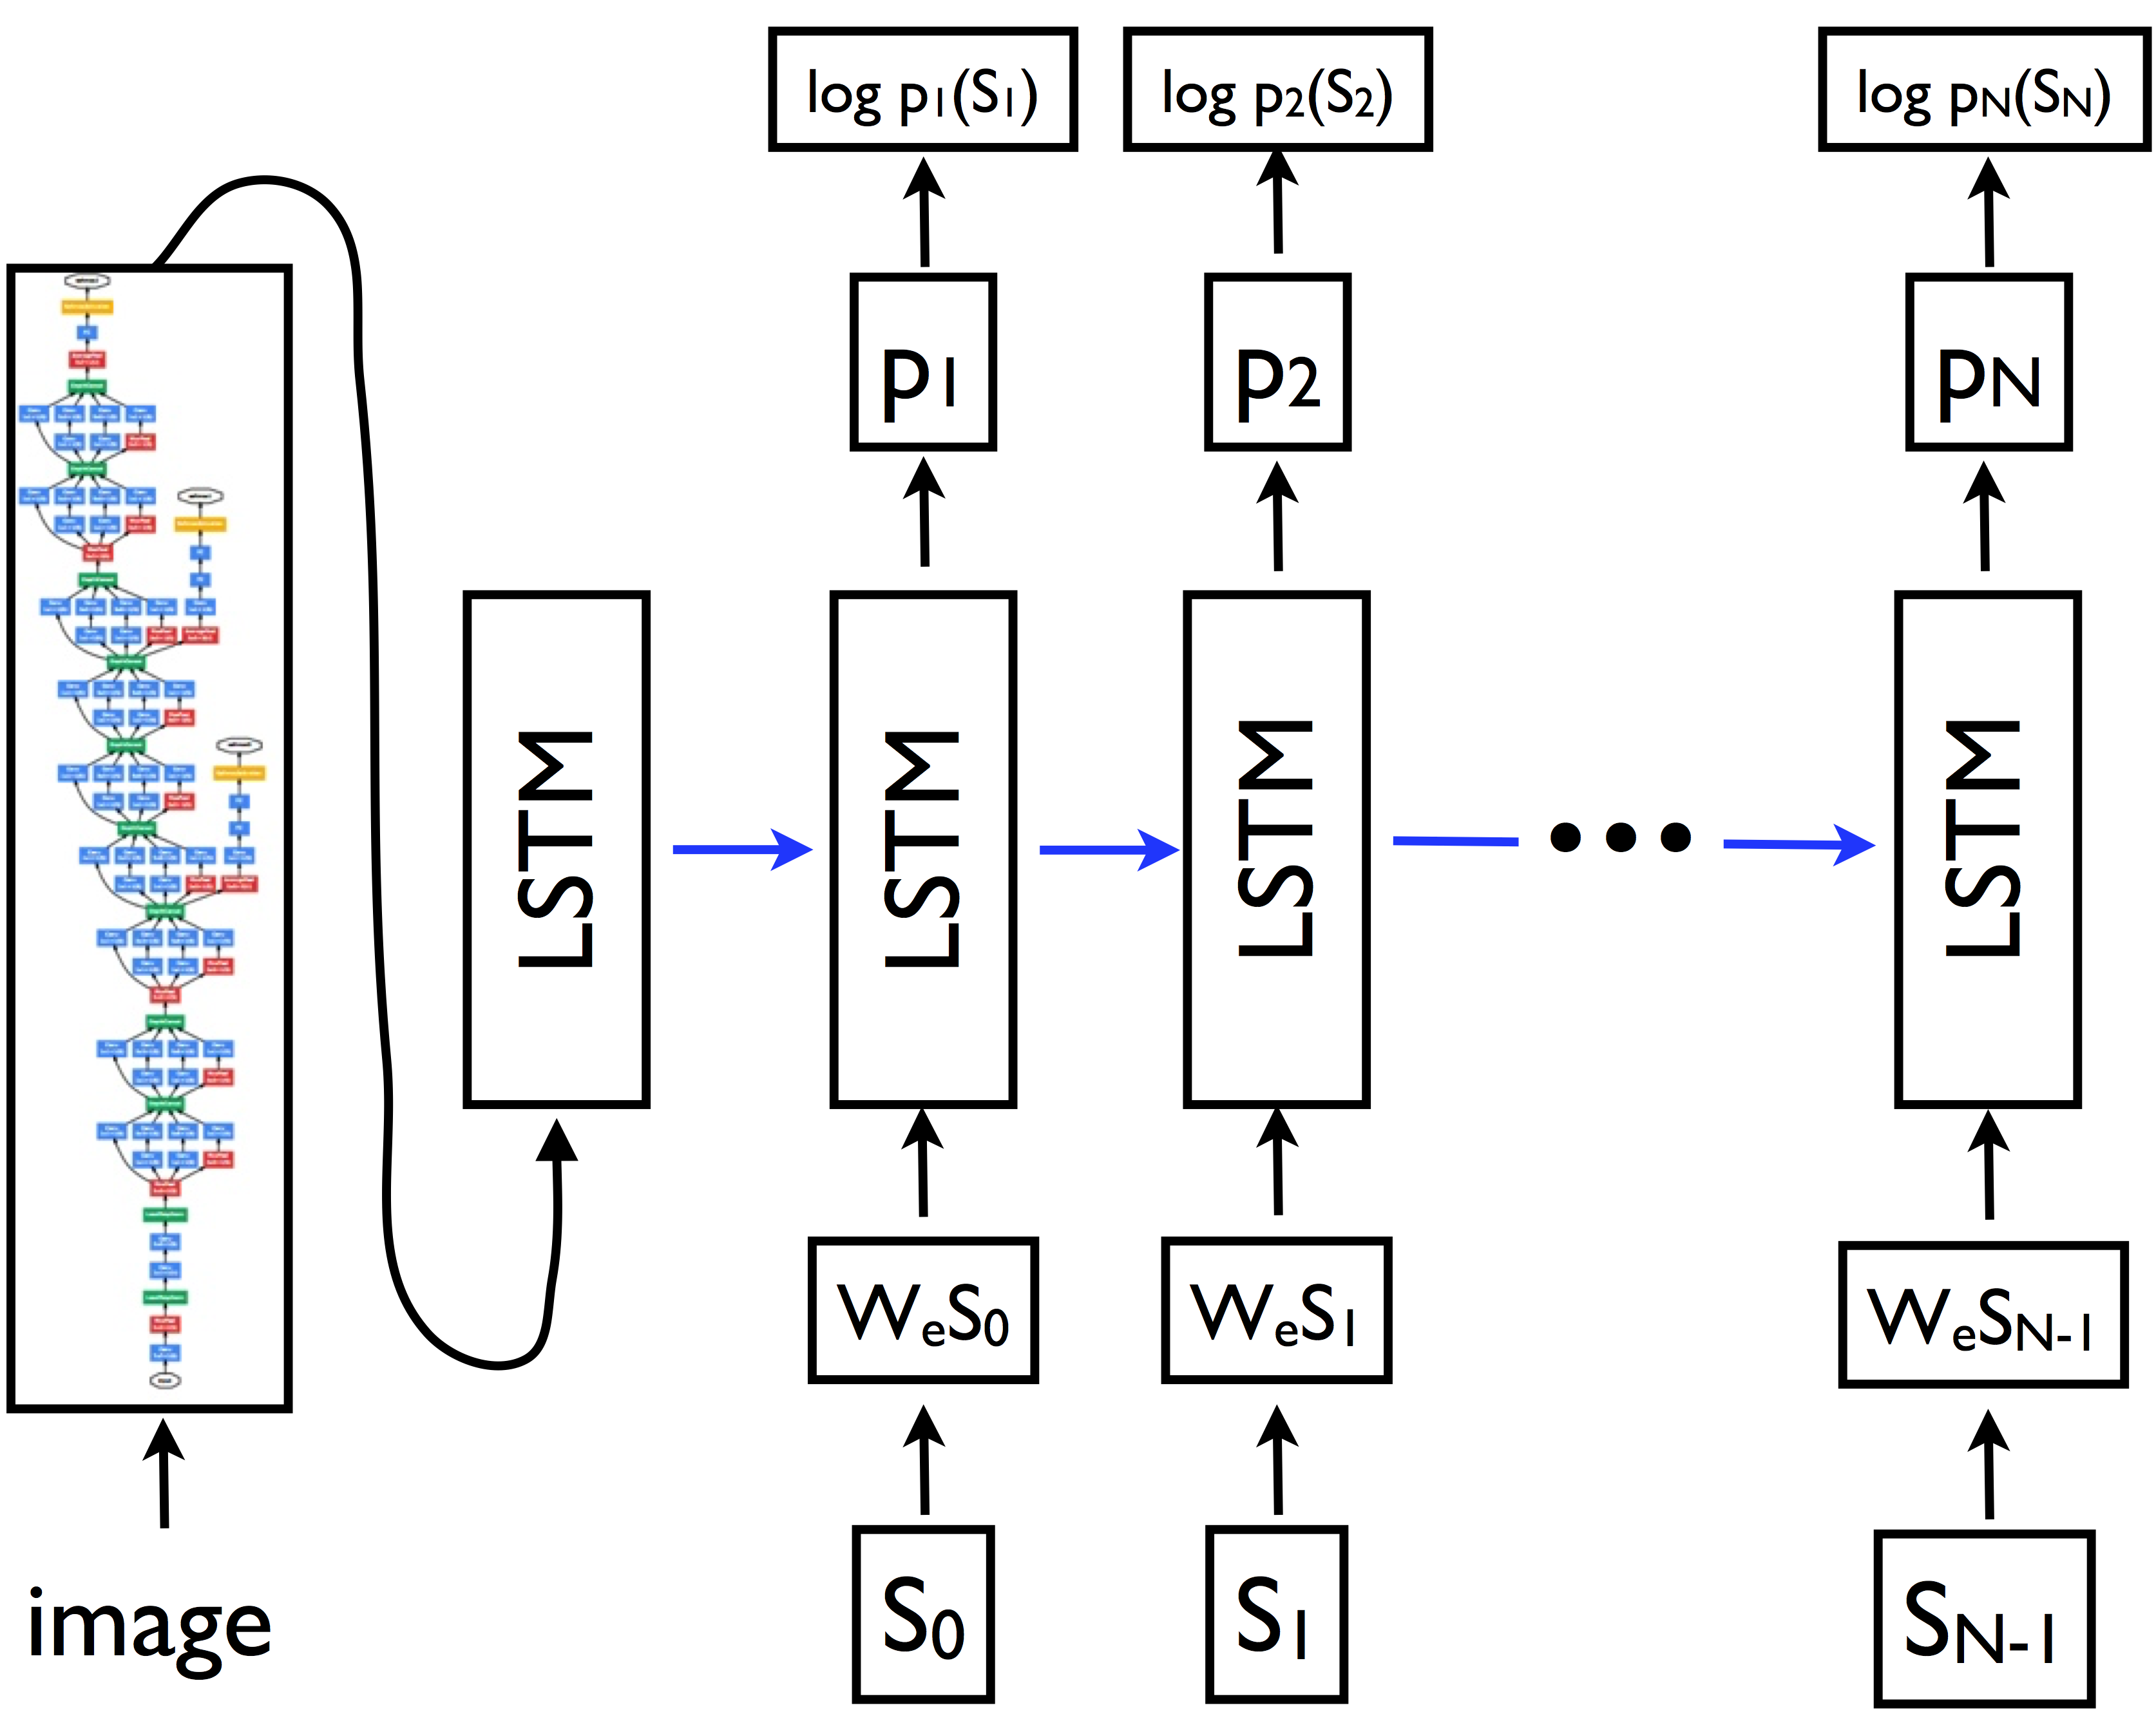
\includegraphics[width=0.9\textwidth]{show_and_tell_architecture}
  \caption{La arquitectura \emph{Show and Tell}, propuesta por Vinyals, \emph{et al},\cite{DBLP:journals/corr/VinyalsTBE14}
    en la cual se conecta una CNN Inception con una LSTM.
    (Tomado de \url{https://arxiv.org/pdf/1411.4555.pdf}.)}
  \label{show_and_tell_architecture}
\end{figure}

\chapter{Experimentación y evaluación del desempeño de la red}
\chaptermark{Experimentación y evaluación}

\noindent
\lettrine[lines=2, lhang=0.33, loversize=0.25]{\textbf{E}}{n}\
este capítulo se detallarán los experimentos hechos con la arquitectura expuesta\
anteriormente. La metodología llevada a cabo consistió en reunir la mayor cantidad\
posible de datos para seguir con los procedimientos descritos en la Sección \ref{sec:arq-accion}.\
Los alcances de los experimentos serán descritos más adelante, dejando en claro\
las restricciones de tiempo (para la realización de la tesis) y capacidad de equipo\
de cómputo disponible.\par
Con respecto a lo último mencionado, para los cómputos de mayor desempeño se utilizó una\
\textbf{tarjeta gráfica} (\emph{GPU}, por sus siglas en inglés) \emph{GeForce GTX 1080 Ti}\
de la marca \emph{NVIDIA}\footnote{
  Para mayor información con respecto al modelo \emph{GeForce GTX 1080 Ti},\
  consultar el sitio \url{http://la.nvidia.com/graphics-cards/geforce/pascal/la/gtx-1080-ti}.
}. Es común que en aprendizaje profundo se usen este tipo de componentes, que originalmente\
se construyen para el mundo de los videojuegos.

\section{Estructura del conjunto de datos} \label{sec:dataset}

\noindent
Como ya fue mencionado anteriormente, los datos se obtuvieron del sitio \verb+MemeGenerator.net+%
\footnote{\url{https://memegenerator.net}}.\
La información recabada en este sitio es reunida a través de usuarios alrededor del mundo,\
quienes de manera libre tienen la posibilidad de generar un nuevo meme. El sitio, además,\
agrupa a los memes en personajes (Figura \ref{meme-characters}) y los jerarquiza en base a\
su popularidad%
\footnote{
  Más aún, cualquier usuario puede crear libremente un personaje nuevo, lo que habilita la idea de\
  buscar y agrupar los memes de acuerdo a su personaje.
}.\par
En total se reunieron \textbf{4379} personajes del sitio web antes mencionado. Por cada uno de ellos\
el número de leyendas usadas para entrenar varía según los resultados obtenidos en cada experimento.\
Considerando que es necesario dividir un conjunto de datos en subconjuntos de entrenamiento y\
validación%
\footnote{
  Usualmente esta división se realiza muestreando aleatoriamente del $70$ al $80\%$ de los datos\
  para entrenamiento y del $30$ al $20\%$ para validación.
}, podemos afirmar que el tamaño de los datos de entrenamiento es pequeño en relación a otros\
conjuntos como \emph{ImageNet}.

\begin{figure}[h]
  \centering
  \begin{minipage}[l]{0.3\linewidth}
    
\includegraphics[width=\linewidth]{meme1}
  \end{minipage}\hfill
  \begin{minipage}[r]{0.3\linewidth}
    
\includegraphics[width=\linewidth]{meme2}
  \end{minipage}\hfill
  \begin{minipage}[r]{0.3\linewidth}
    
\includegraphics[width=\linewidth]{meme3}
  \end{minipage}
  \begin{minipage}[r]{0.3\linewidth}
    
\includegraphics[width=\linewidth]{meme4}
  \end{minipage}\hfill
  \begin{minipage}[r]{0.3\linewidth}
    
\includegraphics[width=\linewidth]{meme5}
  \end{minipage}\hfill
  \begin{minipage}[r]{0.3\linewidth}
    
\includegraphics[width=\linewidth]{meme6}
  \end{minipage}
  \begin{minipage}[r]{0.3\linewidth}
    
\includegraphics[width=\linewidth]{meme7}
  \end{minipage}\hfill
  \begin{minipage}[r]{0.3\linewidth}
    
\includegraphics[width=\linewidth]{meme8}
  \end{minipage}\hfill
  \begin{minipage}[r]{0.3\linewidth}
    
\includegraphics[width=\linewidth]{meme9}
  \end{minipage}
  \caption{
    Ejemplos de personajes populares del sitio \url{https://memegenerator.net}.
    La mayoría de ellos gozaba de gran popularidad entre los años 2009 y 2013;
    la evolución de la viralidad de los mismos y el surgimiento de otros sitios web
    para compartir memes son algunas causas que pueden explicar su ``extinción''.
    (Tomado de \url{https://memegenerator.net}.)
  }
  \label{meme-characters}
\end{figure}

Mediante una búsqueda \emph{por profundidad}, a través del árbol de páginas web, definido por cada uno de los personajes\
del sitio, uno encuentra una gran cantidad de leyendas separadas de la imagen de su personaje asociado.\
Es decir, por cada personaje se extrae una imagen y tantas leyendas como sea posible (Figura \ref{meme-separation}).\par
Para llevar a cabo este fin, se programó un \textbf{rastreador web} (\emph{web crawler}) para llevar a cabo\
la búsqueda de la información y la acumulación de los datos. Se escribió un programa en el lenguaje de\
programación \textbf{Python} (versión 3.6)\footnote{\url{https://www.python.org}} con la biblioteca\
\textit{Scrapy} (versión 1.4.0)\footnote{\url{https://scrapy.org}}, la cual organiza hilos de ejecución concurrentes\
para obtener el contenido de las \verb+URL+'s necesarias mediante peticiones \verb+GET+ de \verb+HTTP+.\
Al final, se organizaron los datos bajo la jerarquía presente en la Figura \ref{file-hierarchy}.

\begin{figure}[h]
  \centering
  \begin{minipage}[l]{\linewidth}
    \dirtree{%
      .1 personaje-1/.
      .2 personaje-1{.}csv.
      .2 personaje-1{.}jpg.
      .2 personaje-1-metadata{.}csv.
      .1 personaje-2/.
      .2 personaje-2{.}csv.
      .2 personaje-2{.}jpg.
      .2 personaje-2-metadata{.}csv.
      .1 {.}.
      .1 {.}.
      .1 {.}.
      .1 personaje-n/.
      .2 personaje-n{.}csv.
      .2 personaje-n{.}jpg.
      .2 personaje-n-metadata{.}csv.
    }
  \end{minipage}
  \caption{
    Como se observa, los datos se guardaron bajo el formato \texttt{CSV}, asociando cada leyenda con la \texttt{URL}
    de su meme asociado y su idioma de origen (Figura \ref{meme-file}). Se estima que un $90\%$ de datos está en inglés.
  }
  \label{file-hierarchy}
\end{figure}

\begin{figure}[H]
  \centering
  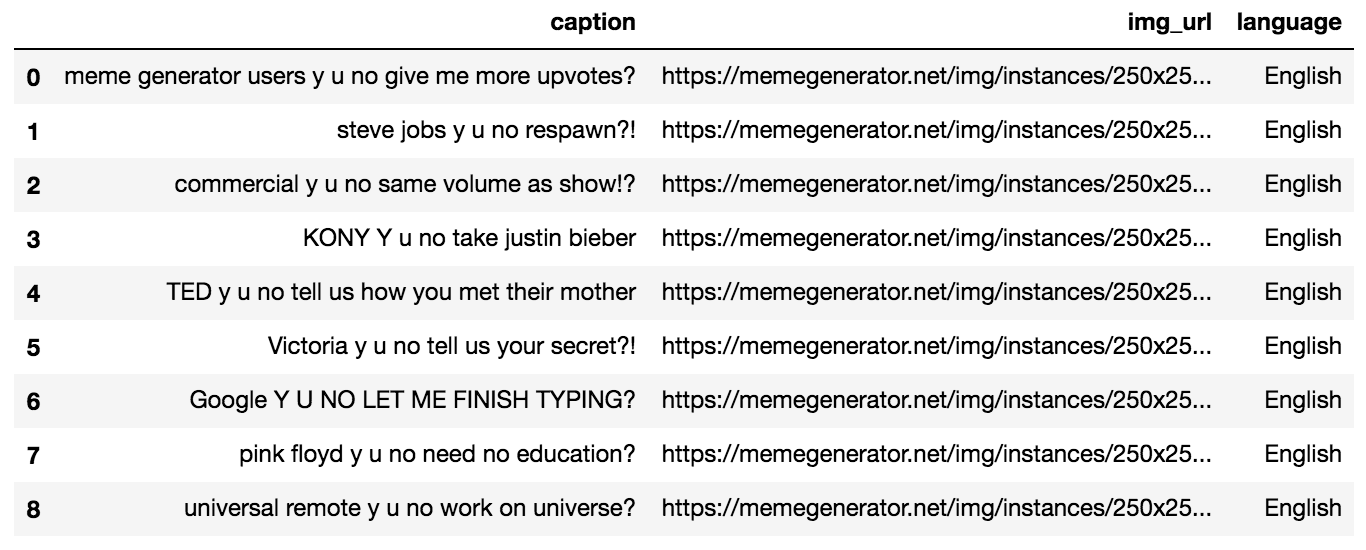
\includegraphics[width=\textwidth]{meme-file}
  \caption{
    De esta manera se guardaron cada una de las leyendas de cada personaje.
  }
  \label{meme-file}
\end{figure}

\begin{figure}
  \centering
  \begin{minipage}[l]{\linewidth}
    
\includegraphics[width=\linewidth]{thesis-i-demand-trial-by-combat}
  \end{minipage}\hfill
  \begin{minipage}[r]{0.5\linewidth}
    
\includegraphics[width=\linewidth]{tyrionlannister}
  \end{minipage}\hfill
  \begin{minipage}[r]{0.5\linewidth}
    \verb+thesis  i demand trial by combat+
  \end{minipage}
  \caption{
    La ilustración de la parte superior constituye a un meme que integra a un personaje con su leyenda y
    es el objeto que se propaga a través de Internet. Los datos que se reunieron se separaron como se
    indica en la ilustración de la parte inferior.
    (Tomado de \url{https://memegenerator.net}.)
  }
  \label{meme-separation}
\end{figure}

\section{Generación de leyendas}

\noindent
El modo \verb+inferencia+ del modelo consiste en generar una leyenda para una imagen de entrada.\
Dada la manera con la cual se representa el modelo de lenguaje aprendido del conjunto de datos\
de entrenamiento, sabemos que por cada palabra hay una distribución de probabilidad que evalúa\
qué tan viable es que cada palabra del vocabulario sea la que sigue. Por lo tanto, muchas veces\
conviene observar los $k$ enunciados que \emph{mejor} describen una imagen, maximizando la\
probabilidad conjunta entre cada una de las palabras que los componen (en orden).\par
La \textbf{búsqueda por haces} (\emph{beam search}, en inglés) es un algoritmo que logra calcular\
enunciados de \emph{``máxima verosimimilitud''}. El procedimiento incorpora a un agente cuyo\
objetivo es encontrar el camino de mayor \emph{peso} posible en una máquina de estados, en la cual solo\
tiene conocimiento del estado actual y los pesos para llegar a los vecinos del mismo. La salida\
del algoritmo muestra los $k$ enunciados más viables para cierta imagen. El agente, entonces\
registra de manera paralela las $k$ palabras de mayor probabilidad que sucedan a la palabra anterior.\par
Normalmente, esto se programa mediante $k$ hilos de ejecución en paralelo. Cada uno se inicializa\
aleatoriamente con las $k$ palabras de inicio de mayor probabilidad. En el paso $t$, cada\
hilo vuelve a calcular los $k$ siguientes mejores estados (un total de $k^2$ estados) y, al final,\
el agente se queda con los mejores $k$ para proceder al paso $t+1$. En este caso, se consideraron\
los $k=3$ mejores enunciados para cada imagen.

\section{Experimentos}

\noindent
Los experimentos realizados obedecen a lo sugerido por la teoría presentada en los dos capítulos anteriores.\
Se buscó seguir la metodología sugerida por el \emph{estado del arte} (\cite{DBLP:journals/corr/VinyalsTBE16}).\
Por ello, se eligió trabajar con el lenguaje de programación Python (versión 3.6) y las bibliotecas\
\textbf{Tensorflow} (versión 1.3.0)\footnote{\url{https://www.tensorflow.org}} y \textbf{Keras}\
(versión 2.0.9)\footnote{\url{https://keras.io}}.\par
Ambas bibliotecas son obra \emph{reciente} de la división de código abierto de \emph{Google}.\
\emph{Tensorflow} surgió como una iniciativa para compartir la manera en que dicha empresa despliega\
sus proyectos que involucran aprendizaje profundo. El paradigma que se sigue consiste en definir un\
grafo dirigido de \emph{tensores} como nodos, en el cual fluirá la información\footnote{
  En cada nodo del grafo, se definen \emph{operaciones} (lectura y escritura de archivos, operaciones\
  matriciales, etc.) y se da la posibilidad de especificar si van a correr en un GPU, si se cuenta con uno.
}; acto seguido, se ``compila'' el modelo y se levanta una sesión para ejecutarlo. Así, \emph{Tensorflow}\
utiliza la sintaxis de \emph{Python} para construir redes neuronales en un mayor nivel.\par
Por otro lado, \emph{Keras} se define a sí misma como una interfaz de programación de aplicaciones (\emph{API})\
de alto nivel, que utiliza como motor de ejecución a \emph{Tensorflow}. Es decir, el programador es capaz\
de escribir código que defina una red neuronal y se ejecute secuencialmente. \emph{Keras}, además,\
facilita la tarea de definir un modelo profundo con una sintaxis más amigable que la de \emph{Tensorflow}\
y configura algunos \emph{hiper-parámetros} de ésta, con el fin de facilitar el prototipado de redes neuronales\
profundas.

\subsection{Experimentos exploratorios}

\noindent
Vinyals, \emph{et al} presentan tanto en \cite{DBLP:journals/corr/VinyalsTBE14} como en \cite{DBLP:journals/corr/VinyalsTBE16}\
el \emph{estado del arte} de los modelos neuronales capaces de generar descripciones a partir de imágenes.\
Por ende, el primer paso experimental consistió en replicar el entrenamiento completo, usando el conjunto de datos\
\emph{ImageNet}.\par
Utilizando pesos pre-entrenados%
\footnote{
  \emph{Tensorflow} provee un conjunto de modelos previamente entrenados bajo un subconjunto de\
  \emph{ImageNet} (\url{http://www.image-net.org/challenges/LSVRC/2012/}). Esto ahorra tiempo en la vectorización\
  de imágenes. Para mayor información, consultar el sitio\
  \url{https://github.com/tensorflow/models/tree/master/research/slim\#tensorflow-slim-image-classification-library}.
} de Inception V3, se realizó el proceso de generar un tensor de incrustaciones de las imágenes de ImageNet\
en un espacio vectorial. Acto seguido se alimentó una LSTM con dicho tensor, como memoria inicial, y se\
entrenó utilizando las leyendas asociadas a cada imagen.\par
Dentro de las ventajas consecuentes de este experimento, está el tener una implementación\
de una LSTM para ser entrenada de nuevo, con cualquier memoria inicial. El desempeño del entrenamiento\
se ilustra en la Figura \ref{exp1}. Es importante destacar que, dadas las altas dimensiones con las que\
se trabaja en cada capa, se estima que se requieren alrededor de 1 millón de épocas para que el error\
dado por la entropía cruzada se estabilice en un valor mínimo (este comportamiento es común para la mayoría\
de los experimentos subsecuentes).\par
El objetivo principal de este primer experimento era familiarizarse con el uso de las implementaciones y la\
tecnología necesaria para realizar aprendizaje profundo. Por ende, se decidió dejar a un lado la evaluación\
del desempeño de este modelo neuronal, mediante un conjunto de datos independiente del de entrenamiento y\
validación.

\begin{figure}[H]
  \centering
  \begin{minipage}[c]{\linewidth}
    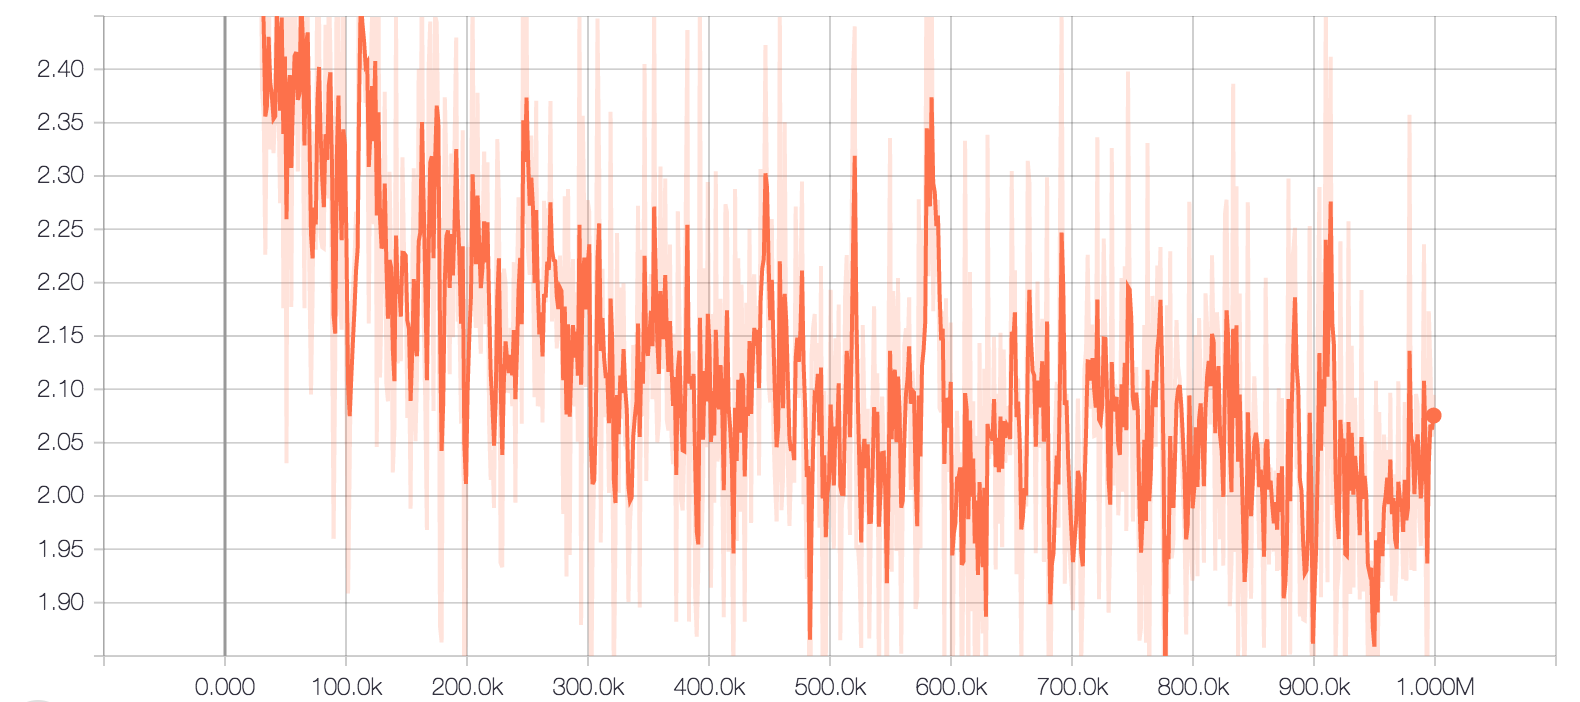
\includegraphics[width=\linewidth]{exp1-1}
  \end{minipage}\hfill
  \begin{minipage}[c]{\linewidth}
    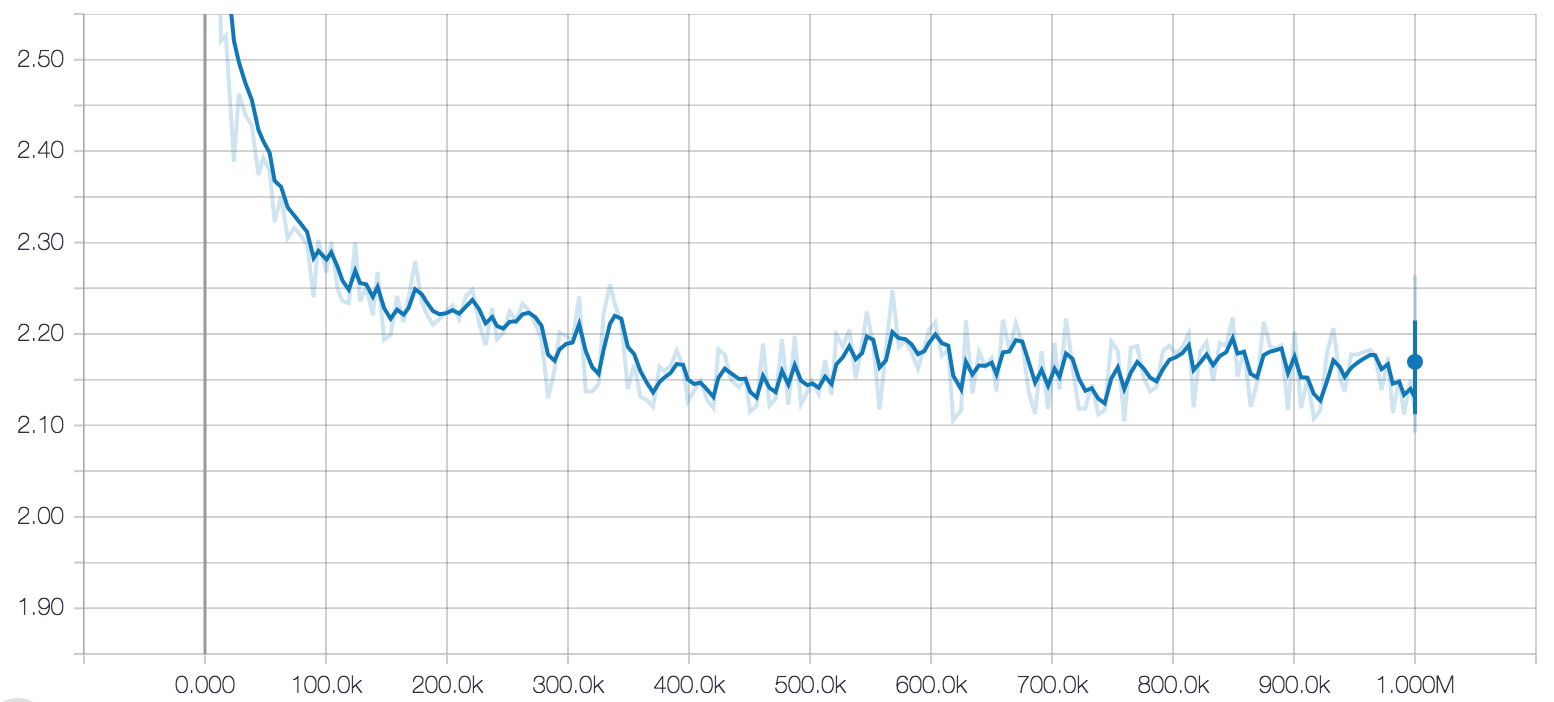
\includegraphics[width=\linewidth]{exp1-2}
  \end{minipage}
  \caption{
    Función de error de entropía cruzada para el primer experimento exploratorio.
    En el gráfico de la parte superior se muestra el error
    a través de cada época del entrenamiento, mientras que el de la parte inferior se
    calculó por medio de un conjunto de datos de \emph{validación} (de menor tamaño que el de entrenamiento).
    Ambos gráficos indican el valor de la entropía cruzada (eje de las ordenadas) a través del
    tiempo (eje de las abscisa).
    (Fuente: elaboración propia.)
  }
  \label{exp1}
\end{figure}

Tenemos, ahora, una CNN que es ``experta'' en etiquetar imágenes con detalles muy generales. Vale la pena,\
entonces, probarla con el conjunto de datos de memes. Buscamos ver, de entrada, que sea capaz de distinguir\
entre dos imágenes distintas (mediante representaciones vectoriales muy diferentes), que además se\
refleje en la discrepancia entre las leyendas generadas. Para ello, diseñamos un experimento en el\
que entrenamos una LSTM con una memoria inicial dada por los códigos convolucionales obtenidos\
a partir de \textbf{97} personajes del conjunto de datos. Estos personajes pasarán por la red\
\emph{Inception V3} pre-entrenada del experimento anterior.

\begin{figure}[h]
  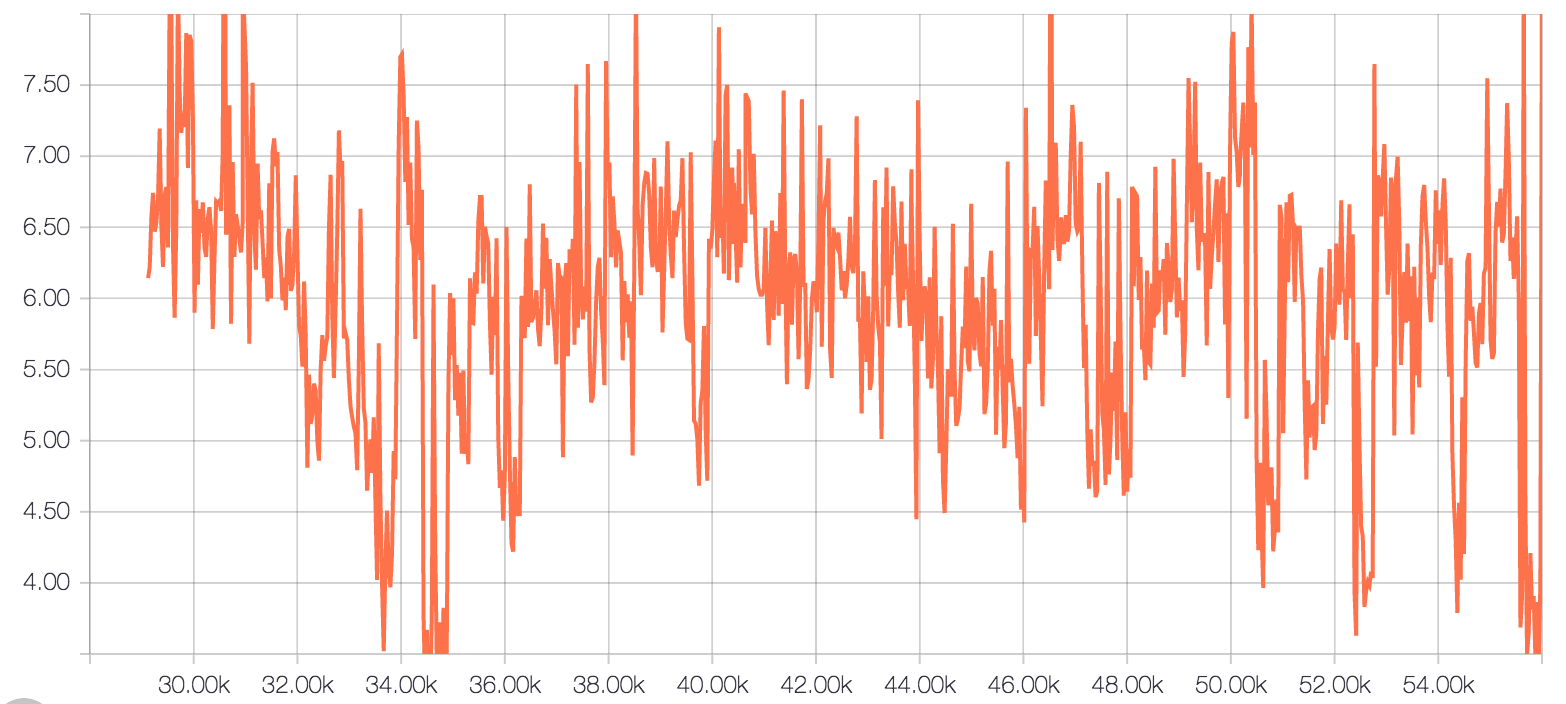
\includegraphics[width=\linewidth]{exp4-1}
  \caption{
    Función de error para el experimento que utiliza la CNN \emph{Inception V3}
    con pesos pre-entrenados, sin ser afinada.
    (Fuente: elaboración propia.)
  }
  \label{exp4}
\end{figure}

Cada personaje posee un promedio de 700 leyendas, pues el número total de leyendas por personaje varía\
según la popularidad del mismo. Cabe destacar que el vocabulario construído tuvo alrededor de 20 mil palabras distintas.\
El desempeño fue deficiente tanto en entrenamiento (Figura \ref{exp4}) como en resultados \emph{anecdóticos}.\
Las siguientes observaciones fueron notables:
\begin{itemize}
\item los códigos convolucionales resultantes del paso por la CNN fueron indistinguibles entre\
  una imagen y otra, dejando en claro la necesidad de realizar una afinación);
\item lo anterior provocó que las leyendas fueran todas iguales para imágenes distintas;
\item el elevado tamaño del vocabulario no favoreció al modelo para poder asignar probabilidades,\
  condicionales, al momento de generar frases (repetición palabras de manera contigua).
\end{itemize}\par
El bajo desempeño de este experimento motivó a \emph{no} realizar una evaluación de los resultados pero\
trajo consigo dos hipótesis para considerarse. La primera de ellas consiste en afinar la red \emph{Inception V3}\
con el conjunto de datos de memes, pues se cree que el modelo implícito en sus parámetros pre-entrenados\
explora detalles mucho más generales de los requeridos para clasificar imágenes como las mostradas en la\
Figura \ref{meme-characters}. Dado el tamaño del conjunto de datos, se plantea, de igual manera, como\
hipótesis, la viabilidad de que una CNN más \textbf{superficial} (menos profunda) tenga éxito al\
generar códigos convolucionales.

\subsection{Experimentos que involucran la afinación de una arquitectura convolucional profunda}

\noindent
Para aprovechar la especialización que posee \emph{Inception V3}, de reconocer patrones simples en\
imágenes, afinamos dicho modelo con un clasificador de memes. Dado que el conjunto de datos\
presentado en la Sección \ref{sec:dataset} no está dividido en ``categorías'' de memes, resulta difícil\
realizar una tarea de aprendizaje supervisado con una CNN.\par
Por otro lado, dadas las características de las imágenes de los memes, existe un patrón más o menos definido\
(rostro del personaje centrado en la imagen) que puede ser explotado contra la tarea general de aprender\
a clasificar \emph{ImageNet}. Esto nos brindó la solución para poder afinar a \emph{Inception V3}: colocar\
una capa MLP, al final de la red, con salida de dos dimensiones para decidir si la entrada es, o no es,\
un meme.\par
Las imágenes \emph{``no memes''} utilizadas en este punto se tomaron aleatoriamente muestreando 4379 de \emph{ImageNet}.\
Se trabajó bajo la premisa de que la profundidad de la red\
alcanzará para generalizar la identificación de las características presentes en un meme. Después de todo,\
nuestro conjunto de datos posee imágenes de mucho menor complejidad que las existentes en \emph{Inception V3}.
En total, se dejaron 3065 imágenes (memes y no memes) para entrenamiento, 657 para validación y 657 para evaluación;
el resultado de este proceso se ilustra en la Figura \ref{exp2}. El desempeño fue bastante favorable,\
ya que se minimizó considerablemente el error de la entropía cruzada. Además, con el conjunto de\
evaluación se corroboró dicho rendimiento mediante los gráficos de las métricas de \emph{precisión}%
\footnote{
  La \textbf{precisión} (\emph{accuracy}, en inglés) puede ser entendida como el porcentaje\
  de aciertos que tiene el modelo al intentar predecir un lote de datos. Se busca, entonces,\
  que su valor esté muy cercano a 1.
} y \emph{error medio absoluto}%
\footnote{
  El \textbf{error medio absoluto} es la diferencia promedio que existe entre los valores\
  estimados por un modelo ($\hat{Y}$) y los valores reales de un conjunto de datos ($Y$). Esto\
  se calcula con la expresión
  \[\frac{\sum_{i=1}^n \hat{Y}_i - Y_i}{n}.\]
} (Figura \ref{eval:exp2}).

\begin{figure}[h]
  \begin{minipage}[c]{\linewidth}
    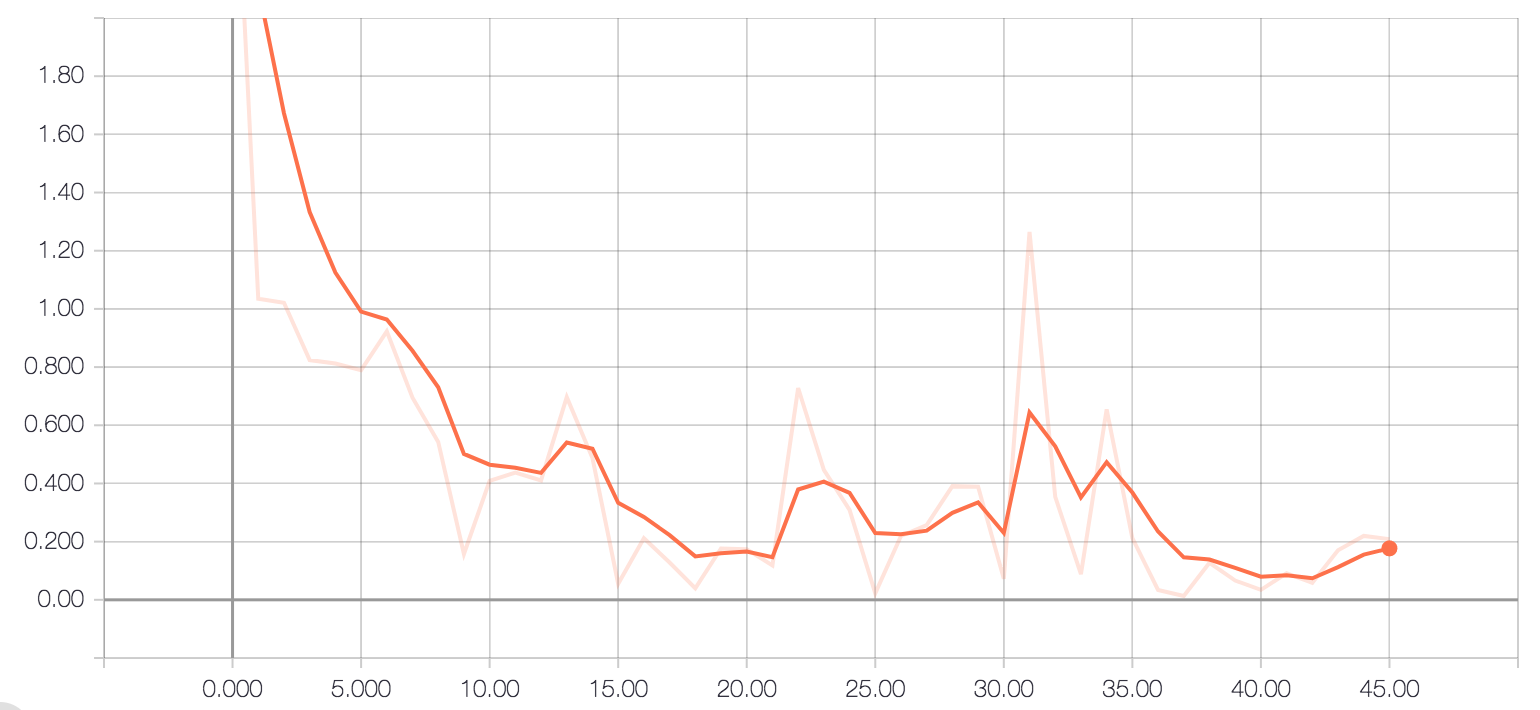
\includegraphics[width=\linewidth]{exp2-1}
  \end{minipage}\hfill
  \begin{minipage}[c]{\linewidth}
    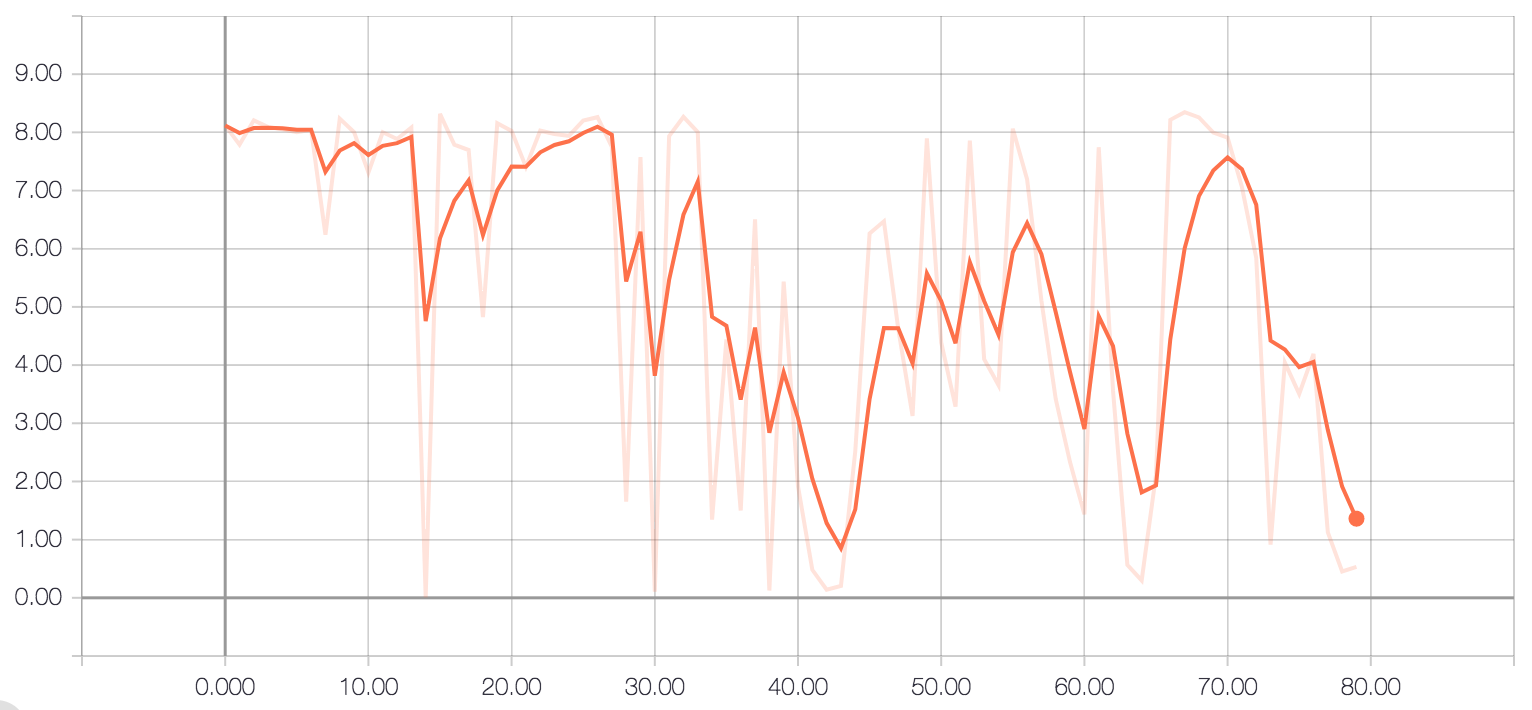
\includegraphics[width=\linewidth]{exp2-2}
  \end{minipage}
  \caption{
    Funciones de error de entrenamiento y validación (gráfico de arriba y de abajo,
    respectivamente) para la afinación de \emph{Inception V3}.
    Esto es, entrenar un clasificador entre lo que es un meme y lo que no es. Se quita\
    la última capa y se añade un MLP con dos dimensiones de salida.
    (Fuente: elaboración propia.)
  }
  \label{exp2}
\end{figure}

\begin{figure}[H]
  \centering
  \begin{minipage}[c]{\linewidth}
    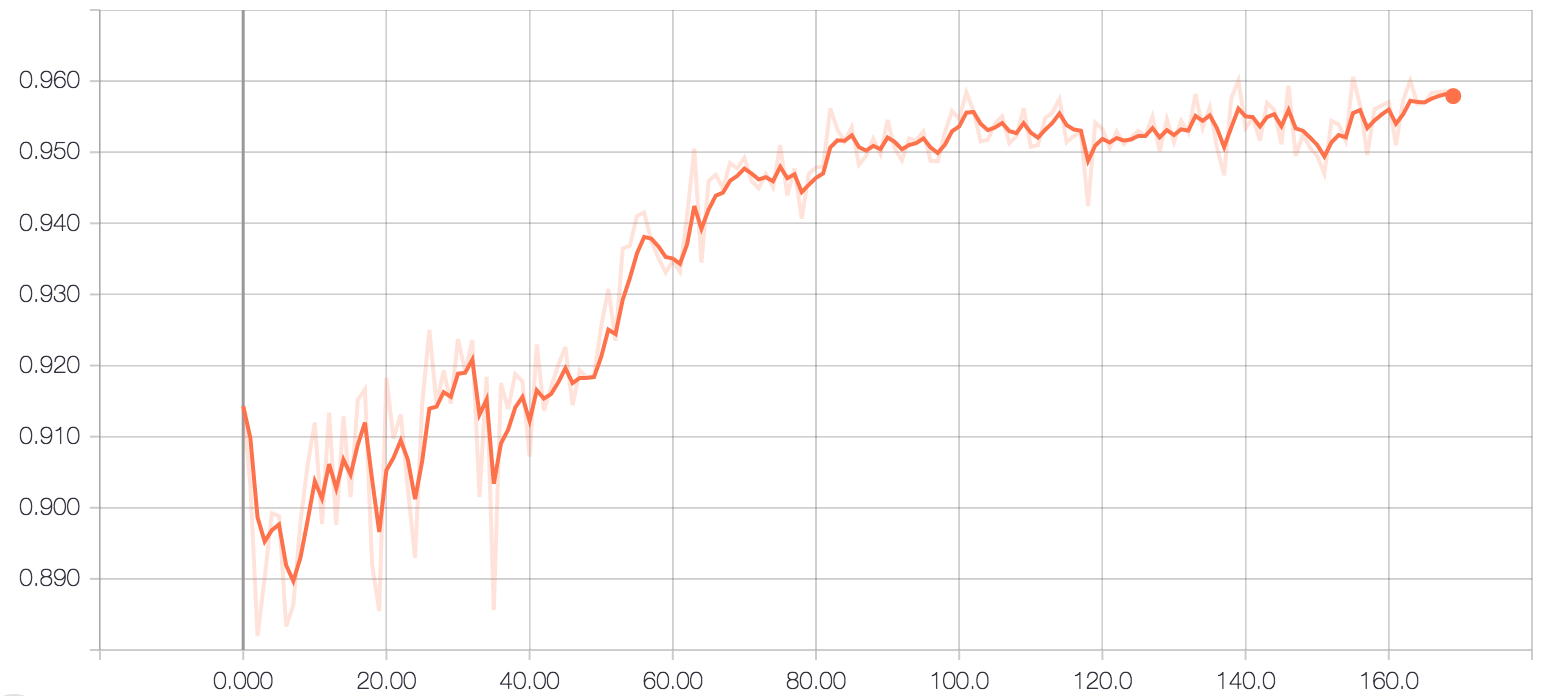
\includegraphics[width=\linewidth]{exp2-3}
  \end{minipage}\hfill
  \begin{minipage}[c]{\linewidth}
    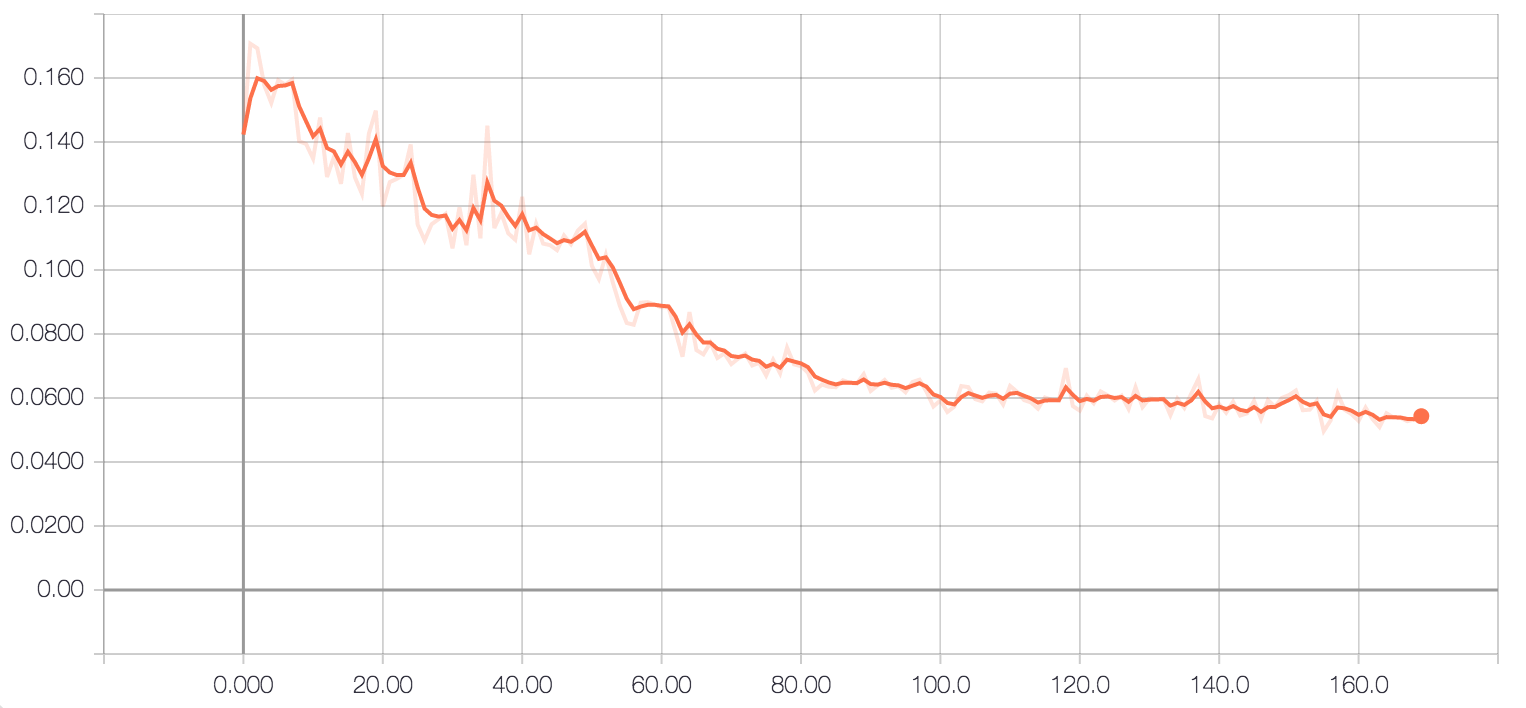
\includegraphics[width=\linewidth]{exp2-4}
  \end{minipage}
  \caption{
    Dos funciones de evaluación para la afinación de \emph{Inception V3}.
    El gráfico de la parte superior muestra la \emph{precisión} con la que el modelo realiza
    sus clasificaciones, mientras que el gráfico de la parte inferior muestra el
    \emph{error medio absoluto} entre las clasificaciones hechas por el modelo contra las verdaderas.
    Ambos gráficos se generaron a partir de un muestreo del $10\%$ de los datos disponibles.
    (Fuente: elaboración propia.)
  }
  \label{eval:exp2}
\end{figure}

Una vez teniendo afinada una red neuronal profunda, surge la inquietud de ver si esto ayuda\
a mejorar el primer experimento en el que se entrenó la LSTM usando memes. Por ello\
se usaron los mismos datos que los que se usaron para dicho experimetno pero\
con la \emph{Inception V3} previamente afinada. Esto provocó que entre cualesquiera\
dos imágenes diferentes, existieran dos códigos convolucionales con valores suficientemente\
distintos; lo que implica que las leyendas generadas serán también distintas.\par
El tensor de imágenes y leyendas de entrada $(I, S)$ se fue construyendo en orden,\
de manera que todas las leyendas de un solo personaje permanecían en posiciones contiguas.\
Dada la cantidad desmedida de leyendas, esto provocó que tras ciertas iteraciones se sobreentrenara\
el modelo sobre un mismo lote. Así, al probar el modo de \verb+inferencia+ del mismo,\
se podía observar claramente una tendencia por repetir la ``manera de hablar'' de un cierto personaje\
(Tabla \ref{exp5:anec}). Iteraciones más tarde, esto cambiaba para que el modelo comenzará a repetir la manera de\
hablar de otro personaje. Una de las evidencias del sobreajuste se ilustra en la Figura \ref{exp5}.\par
A pesar que las leyendas generadas aparentan tener sentido, el sobreajuste que se dio en varios\
momentos del entrenamiento motivó a realizar un mayor trabajo de procesamiento previo. En particular,\
se destaca la importancia de restringir el tamaño del vocabulario, así como de mezclar aleatoriamente\
los tensores de memoria inicial que alimentarán la LSTM. Esta última acción garantiza que no se repitan\
ciertas frases un número de veces elevado en cada lote de entrenamiento, por lo que se espera una\
reducción en el sobreajuste. Por lo tanto, se omitió la evaluación de este experimento, esperando\
resultados más apegados a la realidad de la distribución del conjunto de entrenamiento.

\begin{figure}[h]
  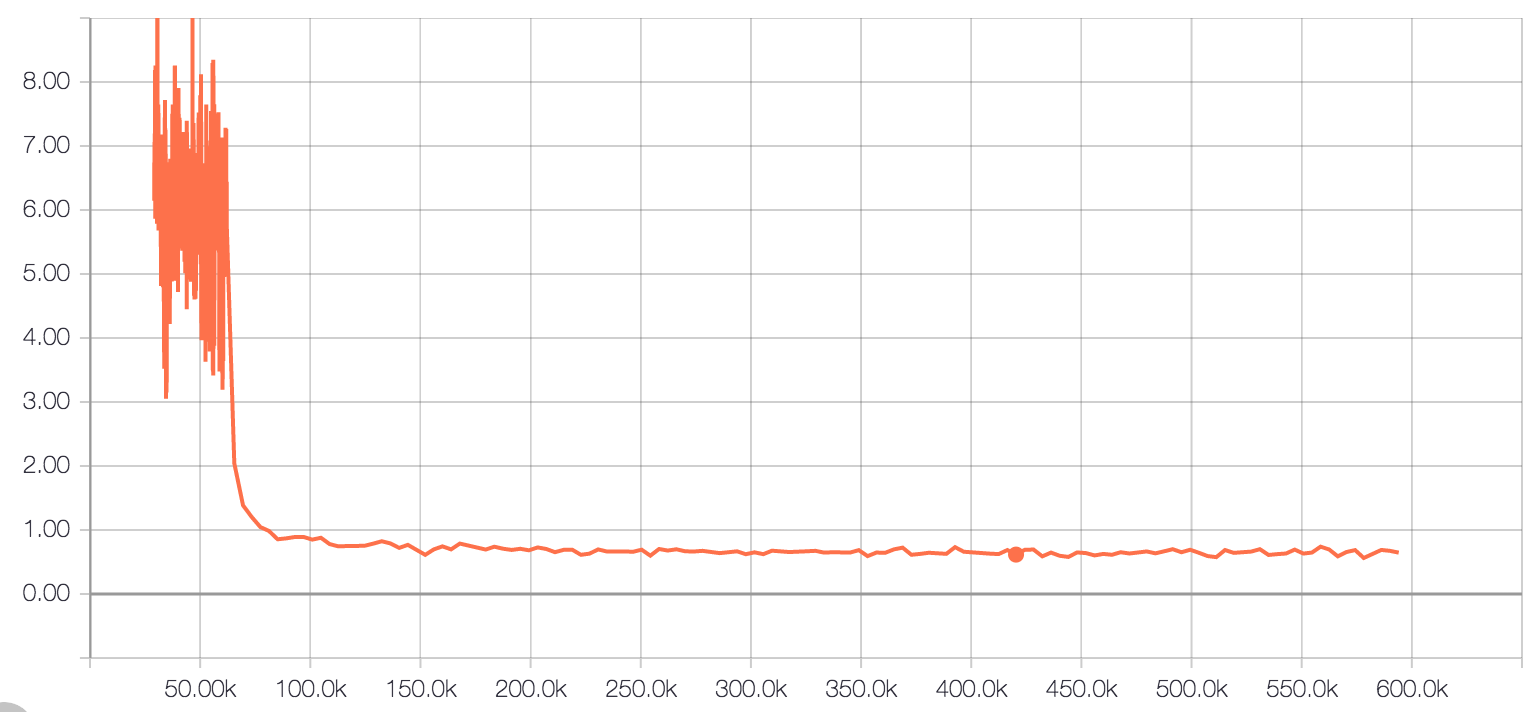
\includegraphics[width=\linewidth]{exp5-1}
  \caption{
    Función de error para el entrenamiento de la LSTM, dándole como estado inicial\
    un tensor generado a apartir de la red \emph{Inception V3} afinada.
    (Fuente: elaboración propia.)
  }
  \label{exp5}
\end{figure}

Para refinar el desempeño de la CNN afinada, el siguiente experimento se diseñó muestreando aleatoriamente\
\textbf{3416} personajes. Además, se eliminaron todas las palabras que no aparecen al menos\
5 veces en todo el conjunto de datos y se usaron únicamente 5 leyendas\
para cada personaje, con el fin de reducir el tamaño del vocabulario. Por consiguiente\
el vocabulario se redujo a 4528 palabras.\par
Previo al entrenamiento, se mezclaron los datos de manera aleatoria en el tensor $(I, S)$;\
esto provocó la diversificación en la manera con la que se generan leyendas para\
imágenes que no aparecen en el conjunto de entrenamiento. El comportamiento de la función de\
error se muestra en la Figura \ref{exp6}.

\begin{figure}[H]
  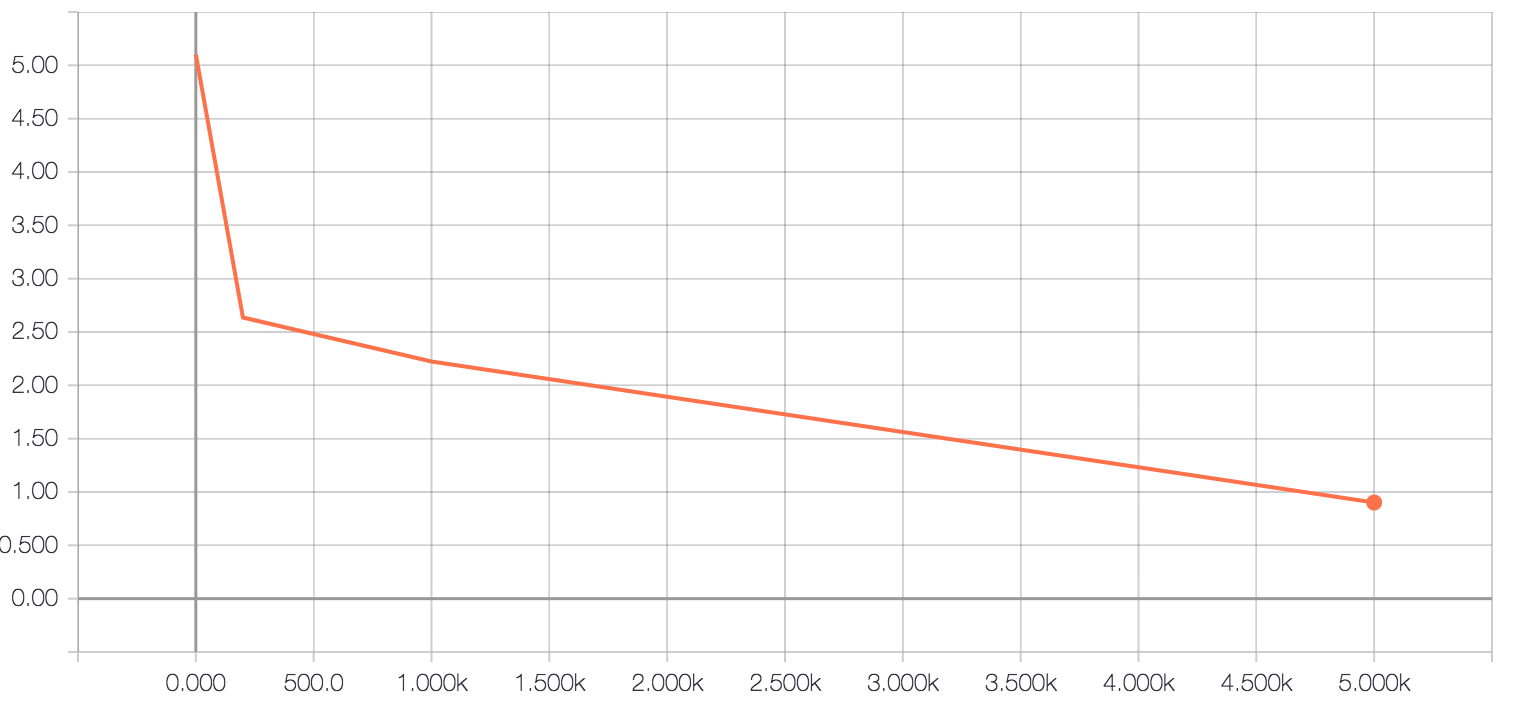
\includegraphics[width=\linewidth]{exp6-1}
  \caption{
    Función de error para el experimento que involucra la red \emph{Inception V3}
    afinada y 5 leyendas por personaje en el entrenamiento.
    (Fuente: elaboración propia.)
  }
  \label{exp6}
\end{figure}

Cualitativamente, la Figura \ref{exp6} muestra una curva descendente más suave, lo que hace pensar\
que el modelo, en efecto, aprendió a generalizar ciertos detalles del conjunto de datos. En promedio,\
podemos afirmar que el error de la entropía cruzada baja, con los cambios hechos y da cierto grado de\
confianza debido a la mezcla aleatoria de las leyendas. Por otro lado, queda la duda de qué pasaría si\
el tensor de códigos convolucionales es generado a partir de una CNN más superficial, algo que es\
válido plantearse debido al número de imágenes disponibles.\par
Este último experimento será el que mejor desempeño trae de los que usaron la red \emph{Inception V3}\
afinada. Efectuar métricas de evaluación como \emph{precisión} y \emph{error medio absoluto} es una\
práctica poco común en tareas que involucran generación de texto: la calidad de las leyendas generadas\
debe ser comparada con un modelo de lenguaje real. Por ello, en la Sección \ref{sec:metrics} presentamos\
una evaluación basada en una métrica común para el procesamiento del lenguaje natural. La Tabla\
\ref{exp6:anec} muestra algunos resultados anecdóticos de este experimento.

\subsection{Experimentos que involucran una arquitectura convolucional superficial}

\noindent
Aunque afinar una CNN profunda, previamente entrenada, es un procedimiento justificado por la literatura,\
el número máximo de imágenes que conforman el conjunto de datos sugiere otro tratamiento.\
Esto indica que entrenar una red neuronal desde cero no es una mala apuesta,\
después de todo, de acuerdo a \cite{DBLP:journals/corr/YosinskiCBL14}.\par
Ahora, presentamos el entrenamiento de una red neuronal superficial (\emph{bastante menos profunda}).\
Se usaron los mismos datos que para la afinación de \emph{Inception V3}.
La arquitectura de esta red se muestra en la Tabla \ref{capas-small},\
el desempeño del entrenamiento se ilustra en la Figura \ref{exp3}, mientras que\
la evaluación del modelo se encuentra en la Figura \ref{eval:exp3}.

\begin{table}[h]
  \resizebox{\textwidth}{!}{
    \begin{tabular}{|l|c|c|}
      \hline
      \textbf{tipo} & \textbf{tamaño de filtro} & \textbf{número de filtros}\\
      \hline \hline
      CONV & $3 \times 3$ & $32$ \\
      \hline
      CONV & $3 \times 3$ & $16$ \\
      \hline
      POOL & $2 \times 2$ & - \\
      \hline
      DROPOUT & $25\%$ de las neuronas se ignoran & - \\
      \hline
      MLP & $128$ unidades de salida & - \\
      \hline
      DROPOUT & $50\%$ de las neuronas se ignoran & - \\
      \hline
      MLP & $2$ unidades de salida & - \\
      \hline
    \end{tabular}
  }
  \caption[Nota al pie]{
    Arquitectura utilizada para entrenar una CNN superficial. Las capas
    \textbf{DROPOUT} constituyen una popular técnica de \emph{regularización}\footnotemark en
    la que se descarta un porcentaje dado de las neuronas de entrada con el fin
    de evitar un sobreajuste sobre el conjunto de datos en cuestión.
  }
  \label{capas-small}
\end{table}

\footnotetext{
  Las técnicas de \textbf{regularización}, en aprendizaje automático, añaden una
  restricción adicional al problema en cuestión para evitar que los valores
  del modelo propuesto se ajusten completamente al conjunto de datos de entrenamiento.
  Es decir, evitar el \emph{sobreajuste} y favorecer la generalización hacia datos
  no observados durante el entrenamiento.
}

\begin{figure}[H]
  \begin{minipage}[c]{\linewidth}
    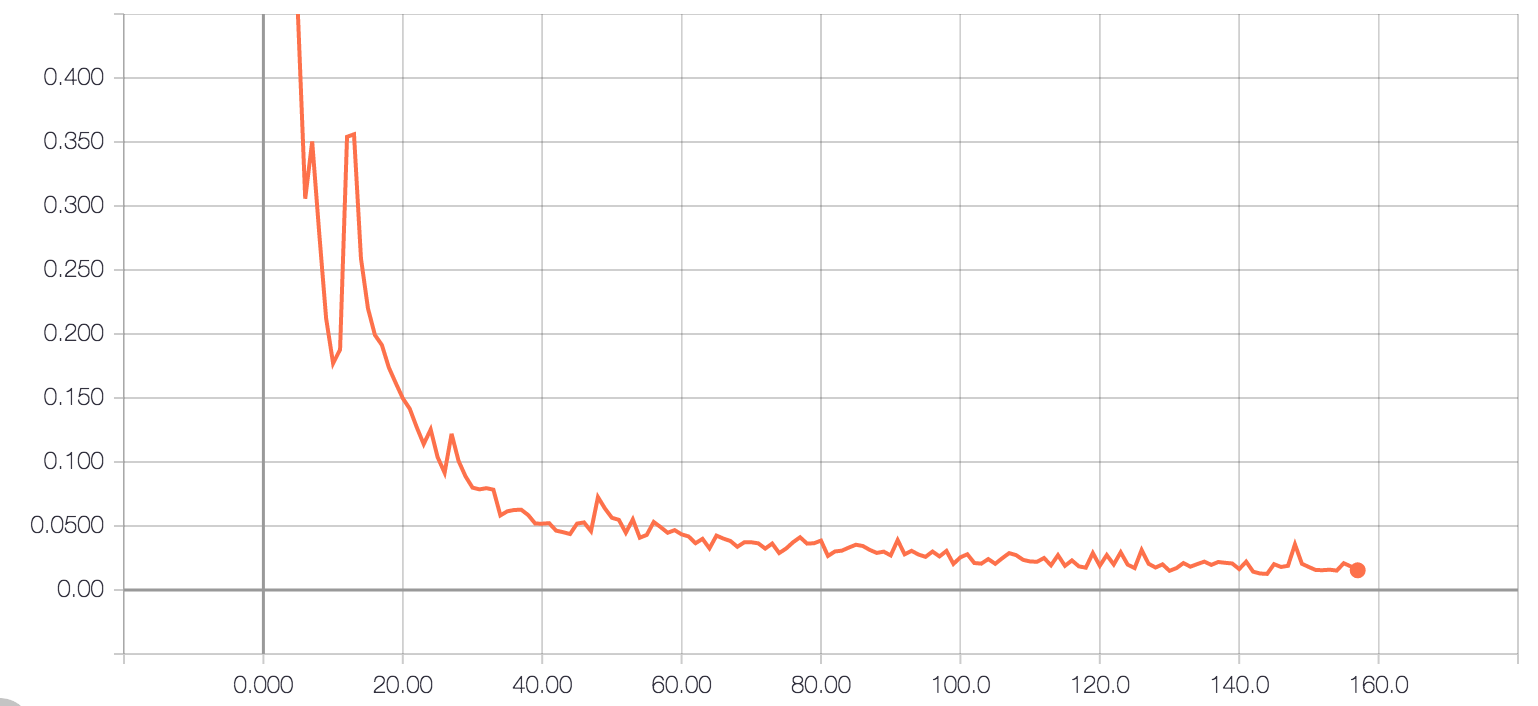
\includegraphics[width=\linewidth]{exp3-1}
  \end{minipage}\hfill
  \begin{minipage}[c]{\linewidth}
    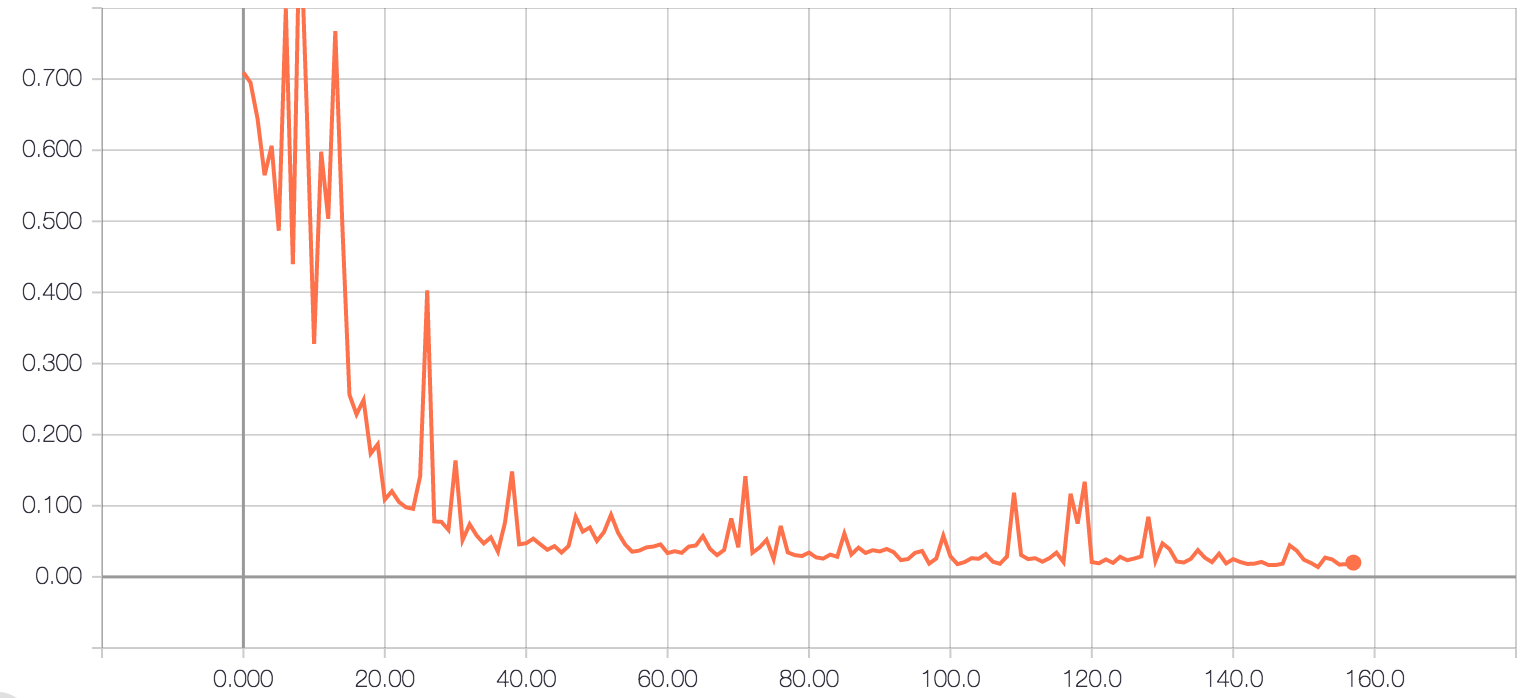
\includegraphics[width=\linewidth]{exp3-2}
  \end{minipage}
  \caption{
    Funciones de error de entrenamiento y validación (gráfico de arriba y de abajo,
    respectivamente) de la CNN superficial. Obsérvese que
    solo se requirieron alrededor de 150 épocas de entrenamiento para llegar a un
    valor óptimo; esto dado el tamaño del conjunto de datos (\emph{memes} y
    \emph{no memes}) que es bastantes órdenes de magnitud más pequeño el\
    conjunto de datos de entrenamiento presentado en la Sección \ref{sec:dataset}.
    (Fuente: elaboración propia.)
  }
  \label{exp3}
\end{figure}

Procedemos, entonces, a replicar el último experimento realizado en la sección anterior.\
Sin embargo, esta vez utilizamos la CNN superficial entrenada sobre memes y no memes.\
El entrenamiento arrojado (Figura \ref{exp7}) fue muy similar a lo observado en la\
Figura \ref{exp6}; no obstante, se logró una mejora en la calidad de las leyendas\
sin ser un detalle anecdótico muy considerable (Tabla \ref{exp7:anec}).

\begin{figure}[H]
  \centering
  \begin{minipage}[c]{\linewidth}
    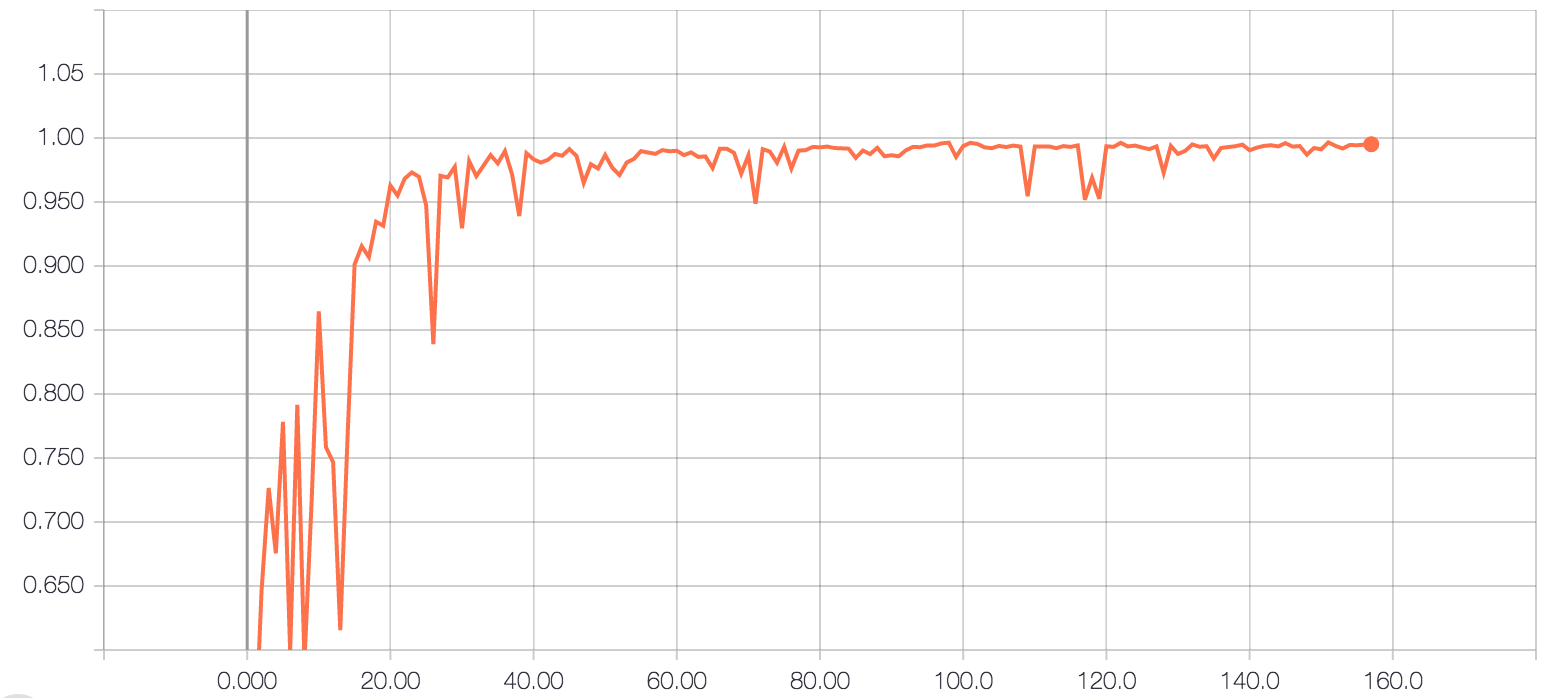
\includegraphics[width=\linewidth]{exp3-3}
  \end{minipage}\hfill
  \begin{minipage}[c]{\linewidth}
    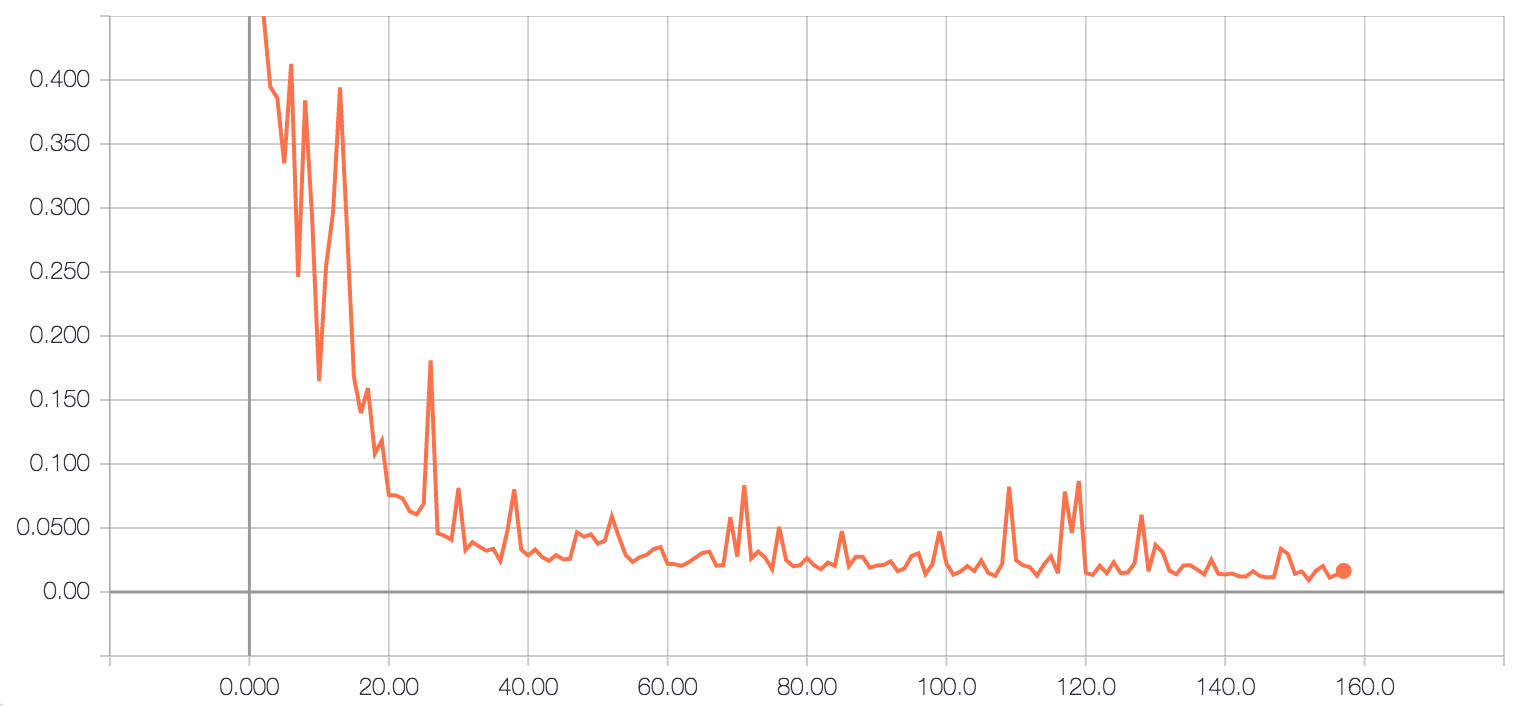
\includegraphics[width=\linewidth]{exp3-4}
  \end{minipage}
  \caption{
    Dos funciones de evaluación para el modelo convolucional superficial.
    El gráfico de la parte superior muestra la \emph{precisión} con la que el modelo realiza
    sus clasificaciones, mientras que el gráfico de la parte inferior muestra el
    \emph{error medio absoluto} entre las clasificaciones hechas modelo contra las verdaderas.
    Ambos gráficos se generaron a partir de un muestreo del $10\%$ de los datos disponibles.
    (Fuente: elaboración propia.)
  }
  \label{eval:exp3}
\end{figure}

Hasta este punto, podemos decir que hemos construido dos modelos convolucionales capaces\
de distinguir entre cualesquiera dos personajes. La tarea pendiente recae en hallar los\
(\emph{híper})-parámetros necesarios para que las leyendas generadas tengan más sentido a juicio\
de un ser humano. Por ello, reportamos un último experimento que involucra un mayor número de palabras\
por personaje.

\begin{figure}[H]
  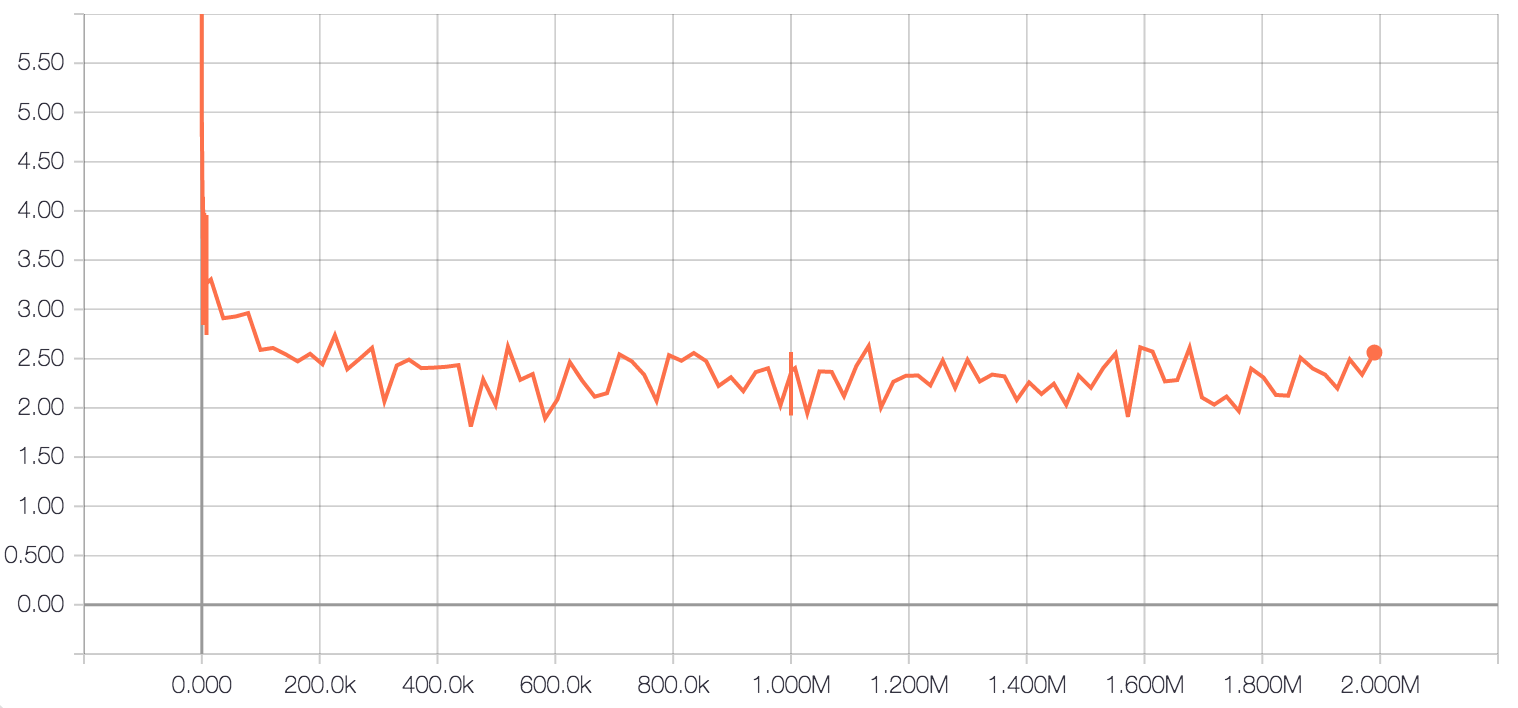
\includegraphics[width=\linewidth]{exp7-1}
  \caption{
    Función de error para el entrenamiento de la LSTM, usando 5 leyendas por personaje,
    un vocabulario reducido y códigos convolucionales generados a partir de una CNN superficial.
    (Fuente: elaboración propia.)
  }
  \label{exp7}
\end{figure}

\begin{figure}[H]
  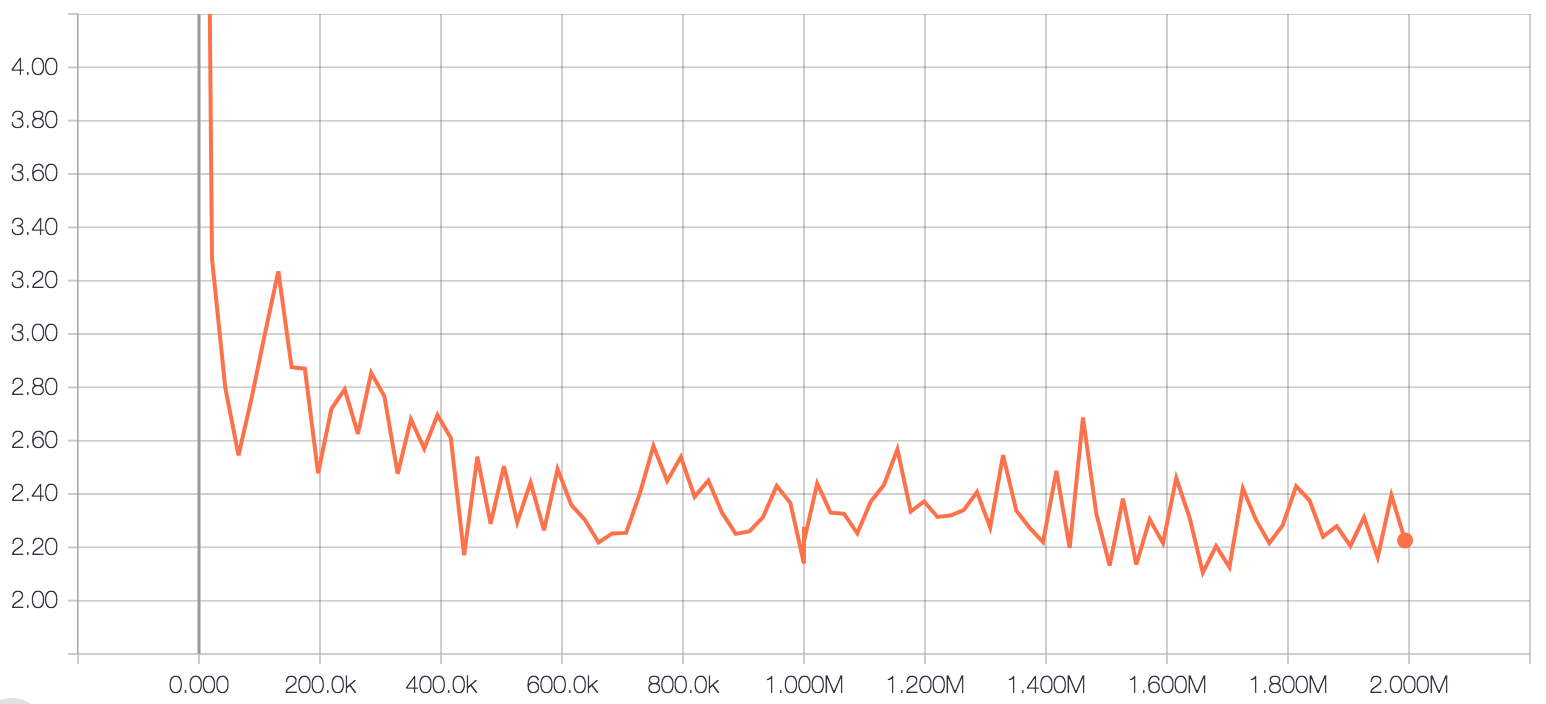
\includegraphics[width=\linewidth]{exp8-1}
  \caption{
    Función de error para el entrenamiento de la LSTM, con códigos convolucionales dados
    por una CNN superficial y 20 leyendas por imagen. Como se observa, existe una ligera
    disminución en el error resultante al final del entrenamiento, con respecto al obtenido
    en experimentos anteriores.
    (Fuente: elaboración propia.)
  }
  \label{exp8}
\end{figure}

Con los mismos datos que para el experimento anterior y con la CNN superficial, se realizó\
el entrenamiento cuyo desempeño se ilustra en la Figura \ref{exp8}. Ahora se aumentó a 20 el\
número de leyendas por imagen. En cuanto a detalles anecdóticos, la Tabla \ref{exp8:anec}\
ilustra una generación de leyendas con un poco de más sentido cuando hay dos palabras\
distintas contiguas. Resumimos los detalles técnicos de todos los experimentos presentados\
en la Tabla \ref{exp-details}.

\begin{table}[H]
  \begin{tabular}{|p{0.5\linewidth}|p{0.2\linewidth}|p{0.3\linewidth}|}
    \hline
    \textbf{tipo de experimento} & \textbf{número de personajes} & \textbf{número de leyendas por personaje}\\
    \hline \hline
    Réplica de entrenamiento de \emph{Inception V3}, como en \cite{DBLP:journals/corr/VinyalsTBE16} & \multicolumn{2}{|c|}{Conjunto de datos \emph{ImageNet}} \\
    \hline
    LSTM a partir de \emph{Inception V3} & 97 & 700, en promedio \\
    \hline
    Afinación de \emph{Inception V3} & \multicolumn{2}{|c|}{3065 memes y 3065 no memes} \\
    \hline
    LSTM a partir de \emph{Inception V3} afinada & 97 & 700, en promedio \\
    \hline
    LSTM a partir de \emph{Inception V3} afinada & 3416 & 5 \\
    \hline
    Entrenamiento de una CNN superficial & \multicolumn{2}{|c|}{3065 memes y 3065 no memes} \\
    \hline
    LSTM a partir de la CNN superficial & 3416 & 5 \\
    \hline
    LSTM a partir de la CNN superficial & 3416 & 20 \\
    \hline
  \end{tabular}
  \caption{
    Resumen de los detalles técnicos presentados en esta sección.
  }
  \label{exp-details}
\end{table}

\section{Evaluación del desempeño de la LSTM} \label{sec:metrics}

\noindent
En el contexto del procesamiento del lenguaje natural, es común preguntarse qué tan \emph{buenos}\
son los enunciados generados con respecto a un lenguaje referencia. En el caso que concierne a esta tesis,\
tratamos con un lenguaje informal, generado a partir de la popularidad que adquieren ciertas frases\
dentro del Internet. Sin embargo, es posible discernir entre un enunciado que hace sentido\
empírico a uno que combina palabras sin patrón alguno.\par
Las métricas propuestas en \cite{DBLP:journals/corr/VinyalsTBE16} sugieren el uso de un corpus\
lingüístico de referencia, con el cual se compare la similitud entre las estructuras gramaticales\
generadas por el modelo con enunciados ``reales''. Por ello, hemos construido un corpus lingüístico
formado por leyendas en el conjunto de \emph{evaluación} para fines de realizar una comparación\
con los resultados emitidos por la LSTM.\par
En particular, analizamos qué tan bien aprende el modelo a predecir la $t$-ésima palabra, a nivel\
probabilístico. Dada la distribución de probabilidad $p$ sobre los enunciados realizados a partir\
de un alfabeto $\Sigma$%
\footnote{
  Es decir, un modelo de lenguaje.
}, definimos la \textbf{perplejidad} $PP(S)$ del modelo como
\begin{equation}
  PP(S) = p(s_1 s_2 \ldots s_n) ^{-\frac{1}{n}}, \label{eq:perplexity0}
\end{equation}
donde $S = s_1, s_2, \ldots, s_n \in S^*$. Desarrollando la Ecuación \ref{eq:perplexity0},\
tenemos que
\begin{align}
  PP(S) &= \sqrt[n]{\frac{1}{p(s_1 s_2 \ldots s_n)}}\\
  &= \sqrt[n]{\prod_{i=0}^n \frac{1}{p(s_{i+1}\ |\ s_1 s_2 \ldots s_i)}} \label{eq:perplexity1}
\end{align}\par
La Ecuación \ref{eq:perplexity1} se obtuvo aplicando la \emph{regla de la cadena} de las probabilidades\
conjuntas a la predicción de cada palabra $s_i$. Lo que este razonamiento nos indica es que\
minimizar la perplejidad de un enunciado $S$ con respecto a un modelo $p$, es lo mismo que\
maximizar la probabilidad de $S$ bajo $p$.\par
Intuitivamente, la \emph{perplejidad} del modelo nos dice el número de posibles candidatos que tiene\
el modelo para la palabra $s_{i+1}$, dadas $s_1, s_2, \ldots, s_i$. Si la \emph{perplejidad} es minimizada,\
entonces el modelo aprende con éxito a descubrir patrones de secuencias de palabras.\par
Queremos comparar los dos \emph{mejores} modelos entrenados, es decir, el mejor de los que\
codifican imágenes con la arquitectura convolucional superficial contra el mejor de los que\
codifican con \emph{Inception V3}. Llamémoslos \verb+Modelo A+ y \verb+Modelo B+, respectivamente.\
Para exponerlos a un conjunto de imágenes ajenas a los datos de entrenamiento, se tomaron 20 ``nuevos\
memes'' (la mayoría, provenientes de sitios web con gran popularidad actual%
\footnote{
  \url{https://www.reddit.com} y \url{https://me.me}.
}), 20 de las imágenes del conjunto de datos de evaluación\
y 20 imágenes nuevas de \emph{ImageNet} (``no memes''). Esta distinción se hizo con el fin de mostrar\
qué tanto aprendió el modelo acerca de los memes y qué tanto generalizó en detalles.\par
Los promedios de las perplejidades arrojadas por cada experimento de\
evaluación se muestran en la Tabla \ref{avgperplexities}. Observamos que la profundidad de la\
CNN del \verb+Modelo B+ brinda un mejor contexto a la LSTM de los\
atributos que constituyen a la imagen de entrada, por lo que se justifica la discrepancia entre las\
perplejidades del \verb+Modelo A+ y del \verb+Modelo B+.\par
Recordemos que la CNN del \verb+Modelo A+ fue entrenada bajo la tarea de distinguir el conjunto de datos\
de memes con un subconjunto de \emph{ImageNet}. Por ello, muchas abstracciones posiblemente identificadas\
por la CNN del \verb+Modelo B+ no logran ser reflejadas en las salidas de la CNN del \verb+Modelo A+.\
Más aún, como la CNN del \verb+Modelo B+ estuvo previamente entrenada con los datos de \emph{ImageNet},\
de los cuales surgen los ``no memes'', es entendible que dicho modelo haya logrado un desempeño similar con\
``no memes'' y memes de evaluación. En contraste, los nuevos memes constituyen una clase de imágenes que no\
fue parte tanto del pre-entrenamiento como de la afinación del \verb+Modelo B+.\par
Los resultados de la evaluación pueden ser consultados de manera\
interactiva en el \textbf{repositorio de código fuente}%
\footnote{
  El repositorio se encuentra en \url{https://github.com/alorozco53/Deep-Meme-Captioner/blob/evaluate/memes/testing.md}.
} de esta tesis.

\begin{table}[H]
  \centering
  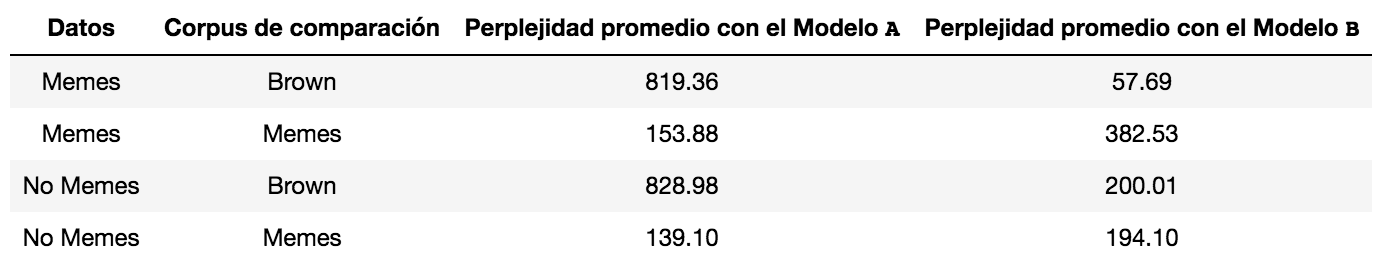
\includegraphics[width=\textwidth]{avgperplexities}
  \caption{
    Promedios de las perplejidades arrojadas al evaluar los dos \emph{mejores} modelos contra el
    \emph{corpus} formado mediante las leyendas de los memes extraídos de Internet.
  }
  \label{avgperplexities}
\end{table}

\chapter{Conclusiones}

TODO


\appendix

\backmatter

\end{document}
